%%%%%%%%%%%%%%%%%%%%%%%%%%%%%%%%%%%%%%%%%
% Beamer Presentation
% Freedom and Distribution - Impression
% Version 1.0 (10/11/12)
%
% This template has been downloaded from:
% http://www.LaTeXTemplates.com
%
% License:
% CC BY-NC-SA 3.0 (http://creativecommons.org/licenses/by-nc-sa/3.0/)
%
%%%%%%%%%%%%%%%%%%%%%%%%%%%%%%%%%%%%%%%%%

%----------------------------------------------------------------------------------------
%	PACKAGES AND THEMES
%----------------------------------------------------------------------------------------

\documentclass{beamer}

\mode<presentation> {

% The Beamer class comes with a number of default slide themes
% which change the colors and layouts of slides. Below this is a list
% of all the themes, uncomment each in turn to see what they look like.

\usetheme{default}
%\usetheme{AnnArbor}
%\usetheme{Antibes}
%\usetheme{Bergen}
%\usetheme{Berkeley}
%\usetheme{Berlin}
%\usetheme{Boadilla}
%\usetheme{CambridgeUS}
%\usetheme{Copenhagen}
%\usetheme{Darmstadt}
%\usetheme{Dresden}
%\usetheme{Frankfurt}
%\usetheme{Goettingen}
%\usetheme{Hannover}
%\usetheme{Ilmenau}
%\usetheme{JuanLesPins}
%\usetheme{Luebeck}
%\usetheme{Madrid}
%\usetheme{Malmoe}
%\usetheme{Marburg}
%\usetheme{Montpellier}
%\usetheme{PaloAlto}
%\usetheme{Pittsburgh}
%\usetheme{Rochester}
%\usetheme{Singapore}
%\usetheme{Szeged}
%\usetheme{Warsaw}

% As well as themes, the Beamer class has a number of color themes
% for any slide theme. Uncomment each of these in turn to see how it
% changes the colors of your current slide theme.

%\usecolortheme{albatross}
%\usecolortheme{beaver}
%\usecolortheme{beetle}
\usecolortheme{crane}
%\usecolortheme{dolphin}
%\usecolortheme{dove}
%\usecolortheme{fly}
%\usecolortheme{lily}
%\usecolortheme{orchid}
%\usecolortheme{rose}
%\usecolortheme{seagull}
%\usecolortheme{seahorse}
%\usecolortheme{whale}
%\usecolortheme{wolverine}

%\setbeamertemplate{footline} 
%\setbeamertemplate{footline}[page number] 

%\setbeamertemplate{navigation symbols}{} 
}

\usepackage{graphicx} % Allows including images
\usepackage{booktabs} % Allows the use of \toprule, \midrule and \bottomrule in tables
\usepackage{hyperref} % Allows the use of hyper text reference
\usepackage{color}    % Allows to color text
\usepackage{tikz}     % Allows to use Tikz PGF
\usepackage{lmodern}  % Allows arbitrary sizing of fonts
\usepackage{textcomp} % Allows use of text symbols
\usepackage{tabularx} % Allows flexible tables




%----------------------------------------------------------------------------------------
%	TITLE PAGE
%----------------------------------------------------------------------------------------

\title[Automotive Storage Battery - Care]{Automotive Storage Battery - Care \\ Lead-Acid for now :)}

\author{Gopal} 
\institute[]
{
Technical Consultant \\
\bigskip
\textit{gopalkrish361957@gmail.com} 
}
\date{\today}

\begin{document}

\begin{frame}
\titlepage 
\end{frame}

\begin{frame}
\frametitle{Overview} 
\fontsize{6pt}{10}\selectfont
\tableofcontents 
\end{frame}

%----------------------------------------------------------------------------------------
%	PRESENTATION SLIDES
%----------------------------------------------------------------------------------------


%------------------------------------------------
\section{Battery - About Me :)}
%------------------------------------------------

{ % all template changes are local to this group.
    \setbeamertemplate{navigation symbols}{}
    \begin{frame}[plain]
        \begin{tikzpicture}[remember picture,overlay]
            \node[at=(current page.center)] {
                
\includegraphics[width=\paperwidth]{./Resources/Images/Hi_Battery.pdf}
            };
        \end{tikzpicture}
     \end{frame}
}

{ % all template changes are local to this group.
    \setbeamertemplate{navigation symbols}{}
    \begin{frame}[plain]
        \begin{tikzpicture}[remember picture,overlay]
            \node[at=(current page.center)] {
                
\includegraphics[width=\paperwidth]{./Resources/Images/I_Work_For.pdf}
            };
        \end{tikzpicture}
     \end{frame}
}

{ % all template changes are local to this group.
    \setbeamertemplate{navigation symbols}{}
    \begin{frame}[plain]
        \begin{tikzpicture}[remember picture,overlay]
            \node[at=(current page.center)] {
                
\includegraphics[width=\paperwidth]{./Resources/Images/Elephant_Blindmen.pdf}
            };
        \end{tikzpicture}
     \end{frame}
}

{ % all template changes are local to this group.
    \setbeamertemplate{navigation symbols}{}
    \begin{frame}[plain]
        \begin{tikzpicture}[remember picture,overlay]
            \node[at=(current page.center)] {
                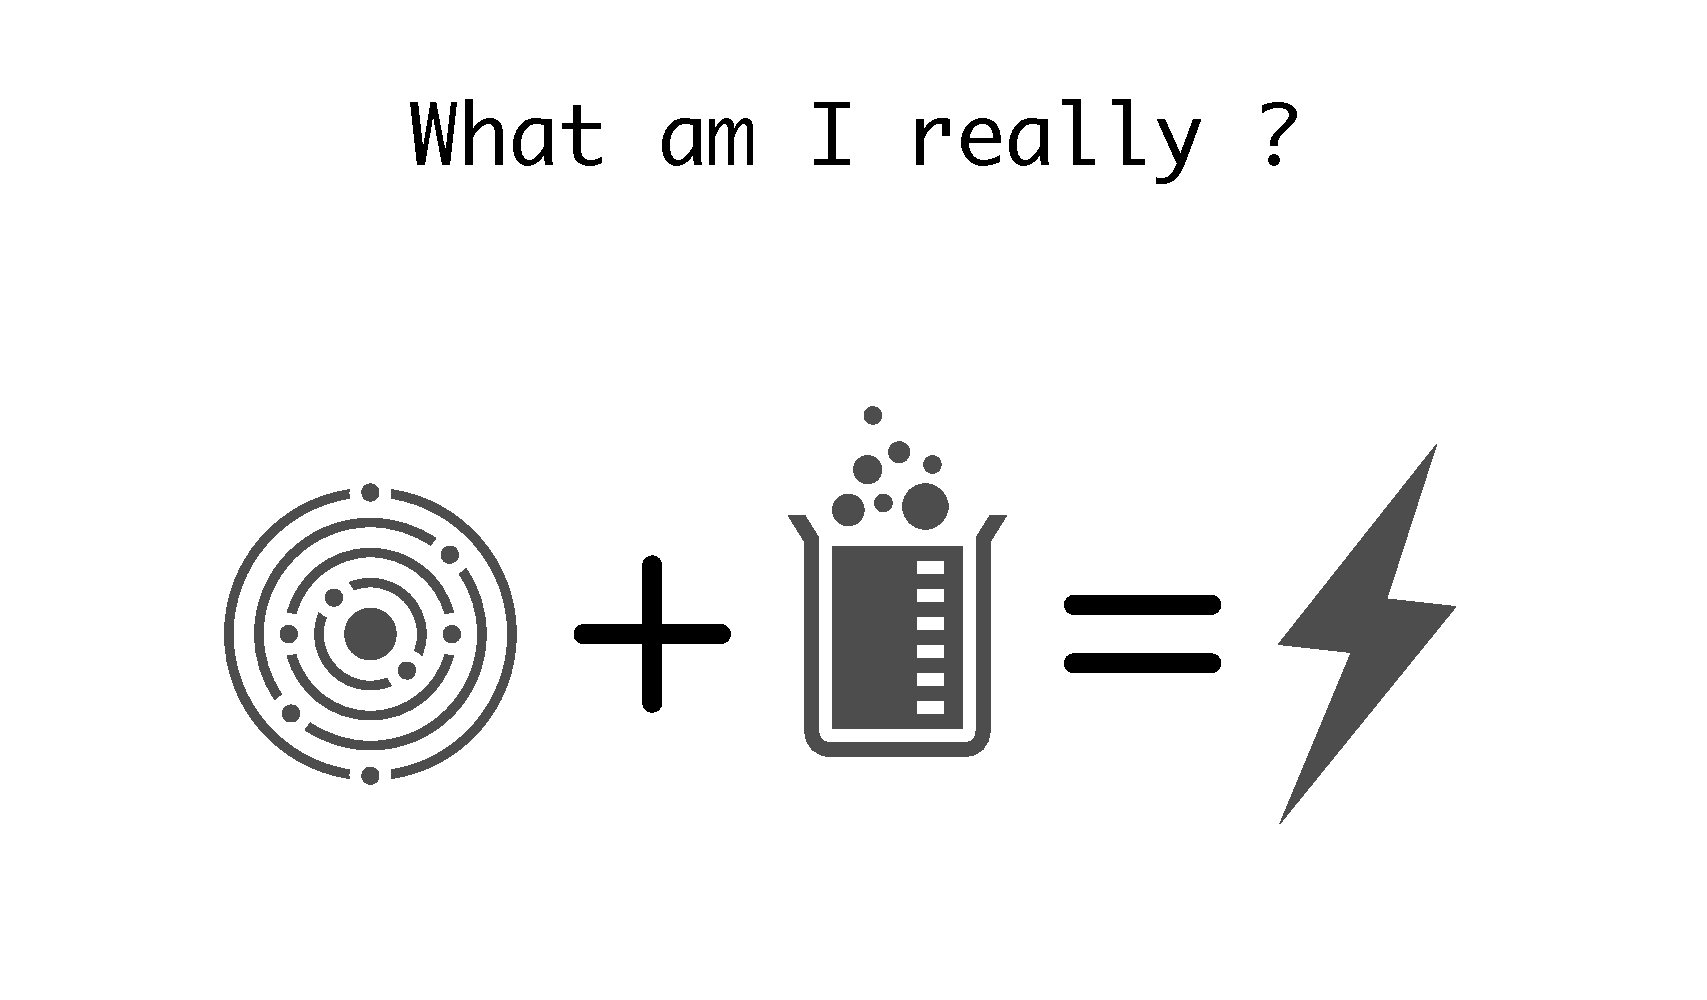
\includegraphics[width=\paperwidth]{./Resources/Images/What_Am_I.pdf}
            };
        \end{tikzpicture}
     \end{frame}
}


%------------------------------------------------
\section{Introduction}
%------------------------------------------------

\begin{frame}   %------SLIDE
  \frametitle{Automobile Electrical system}
  \begin{center}
    It constitutes the essentials of a public electricity supply system ...    
    - - - - - - 
  \end{center}
  \begin{itemize}
    \item \textbf{Generation}   $\equiv$ Dynamo or Alternator
    \item \textbf{Storage}      $\equiv$ Battery
    \item \textbf{Utilization}  $\equiv$ Cranking, Ignition, Starting, lighting, etc...
  \end{itemize}
\end{frame}

\begin{frame}   %------SLIDE
\fontsize{8pt}{4}\selectfont
  \frametitle{Battery}

  \textbf{Use:}
  \begin{itemize}
    \item Battery serves to store electrical energy when there is little demand of current
    \item Acts as Standy Source
  \end{itemize}
  
  \vspace{-10pt}
  \begin{figure}
    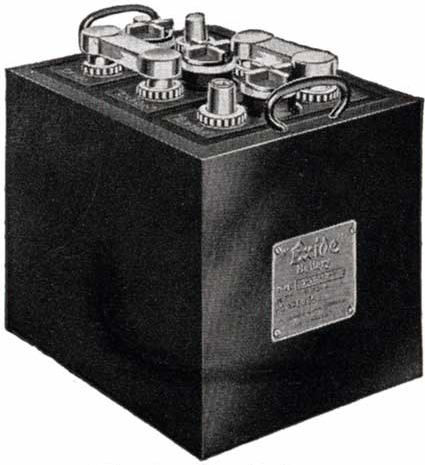
\includegraphics[width=0.20\paperwidth]{./Resources/Images/battery.jpg}
  \end{figure}
  \vspace{-20pt}
    
  \textbf{Calibre:}  
  \begin{itemize}
    \item Robust Construction
    \item Must withstand severe Vibration
    \item Must withstand high charging rates \& heavy discharge currents
  \end{itemize}

  \bigskip
  \textbf{Fact:}
  \begin{itemize}
    \item Not always in accessible location
    \item Not given proper attention
  \end{itemize}  
  
  \begin{center}
    Hence, forms the \textbf{Weak Link} of the Automobile Electrical System
  \end{center}
\end{frame}

\begin{frame}   %------SLIDE
  \frametitle{Principle of Operation}
  \fontsize{8pt}{10}\selectfont
  \begin{center}
    Underlying Principle: \textbf{Electrolysis} \\
    - - - - - - 
  \end{center}

  \textbf{Constituents:}
  \begin{itemize}
    \item \textbf{Electrodes:} Two dissimilar metals.
    \item \textbf{Electrolyte:} Chemical that causes greater chemical change in one of the electrode than in other.
  \end{itemize}
  
  \bigskip
  \textbf{Result:}
  \begin{itemize}
    \item Difference in chemical action $\propto$ Electrical pressure (\textit{a Voltaic Cell})
    \item Electrical Pressure $\equiv$ Electromotive Force
    \item Since the Chemical reaction is reversible, it is a Secondary cell.
  \end{itemize}
  
  \begin{center}
    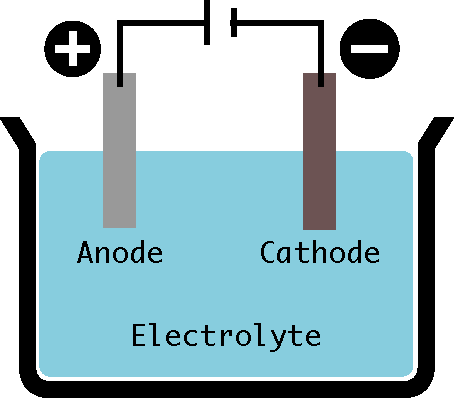
\includegraphics[width=0.2\paperwidth]{./Resources/Images/Electrolysis.pdf}  
  \end{center}
  
\end{frame}



%------------------------------------------------
\section{Construction}
%------------------------------------------------

\begin{frame}     %----SLIDE
  \frametitle{Construction of Automobile Battery}
  \fontsize{8pt}{12}\selectfont
  
  \begin{center}
    A typical automotive battery consists of the following parts:
  \end{center}

  \vspace{-10pt}
  \begin{figure}
    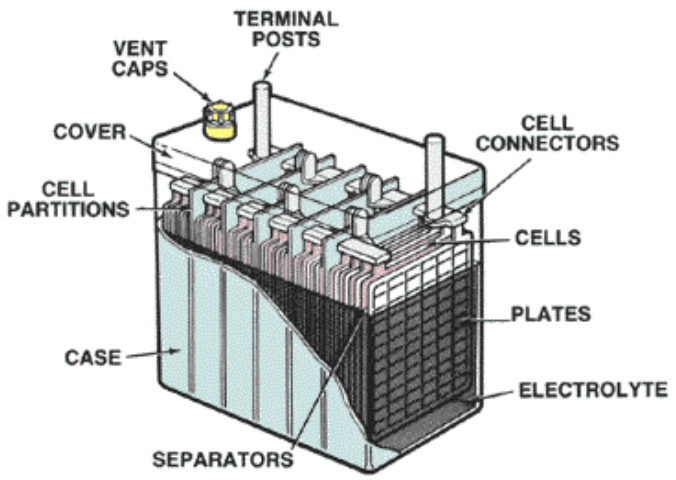
\includegraphics[width=0.4\paperwidth]{./Resources/Images/construction.jpg}
  \end{figure}  
  \vspace{-50pt}
  
  \begin{itemize}
    \item Plates
    \item Separators
    \item Electrolyte
    \item Cell connectors
    \item Vent plug
    \item Cover \& Jar
    \item Battery Case
  \end{itemize}

\end{frame}


\begin{frame}     %----SLIDE
  \frametitle{Plates}
  \fontsize{8pt}{15}\selectfont
  \vspace{-20pt}
  \begin{center}
    Automotive battery plates are formed using \href{https://en.wikipedia.org/wiki/Camille_Alphonse_Faure}{\textit{\textbf{\underline{Faure Process}}}}
  \end{center}
    
    \textbf{Grid:}
    \begin{itemize}
      \item A grid is initially made using Lead \& Antimony.
        \begin{itemize}
          \fontsize{8pt}{15}\selectfont
          \item Mechanical support for the active material.
          \item Enabling the Current Conduction.
        \end{itemize}
      \item \textbf{Positive Plate} : Grid is pasted with mix of Red Pb \& other chemicals pasting, with dilute $H_{2}SO_{4}$
      \item \textbf{Negative Plate} : Grid is pasted with mix of Litharge \& other chemicals pasting, with dilute $H_{2}SO_{4}$      
    \end{itemize}

\end{frame}


\begin{frame}   %----SLIDE
  \frametitle{Plates ...}
  \begin{figure}
    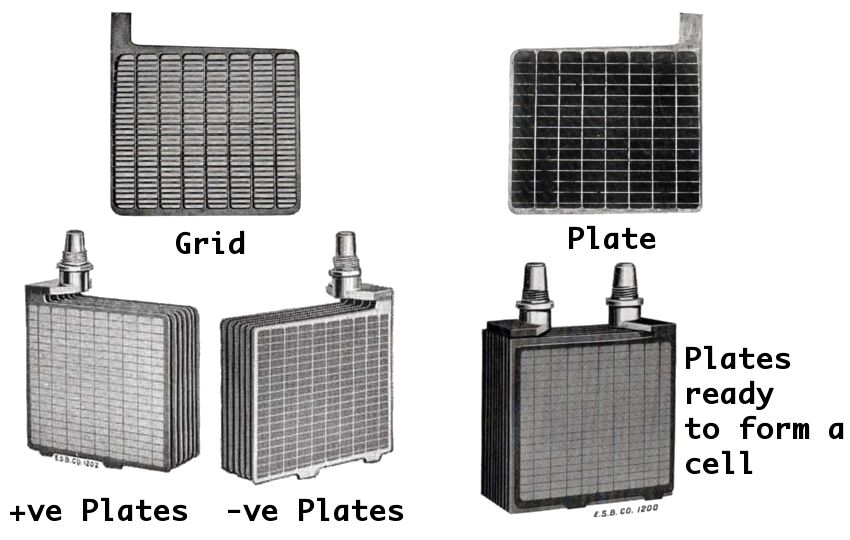
\includegraphics[width=0.8\linewidth]{./Resources/Images/grids_plates_groups.jpg}
  \end{figure}
\end{frame}


\begin{frame}    %----SLIDE
  \frametitle{Separators}
  \fontsize{8pt}{12}\selectfont
    
  \textbf{Functinolity:}
  \begin{itemize}
    \item They are the insulators that prevents short circuiting between $+ve$ \& $-ve$ plates.
    \item They also ease the diffuse of electrolyte in the cell. It is made of PVC or Glass wool.
  \end{itemize}
  
  \begin{figure}
    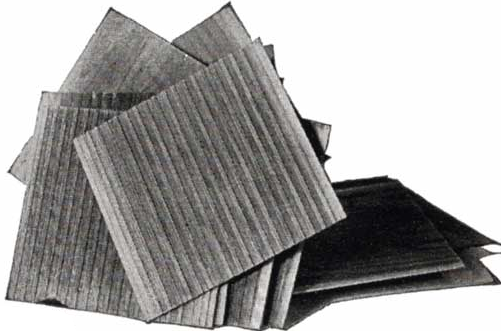
\includegraphics[width=0.6\linewidth]{./Resources/Images/separators.png}
  \end{figure}
\end{frame}

\begin{frame}    %----SLIDE
  \frametitle{Electrolyte}
  \fontsize{7pt}{10}\selectfont
  
  \begin{center}
    Battery electrolyte is a mixture of 36\% $H_{2}SO_{4}$ and 64\% distilled water $H_{2}O$. \\ Today batteries
    have an electrolyte with a Specific gravity of 1270, when fully charged @ 20\textcelsius.
  \end{center}
  
  \textbf{Specific Gravity:} It is the weight of a given volume of liquid in comparison to the weight of the same
  volume of water. The higher the specific gravity of a liquid the denser(thicker) it is. It means \textbf{\textit{exact weight}}.
  
  \vspace{-10pt}
  \begin{center}
    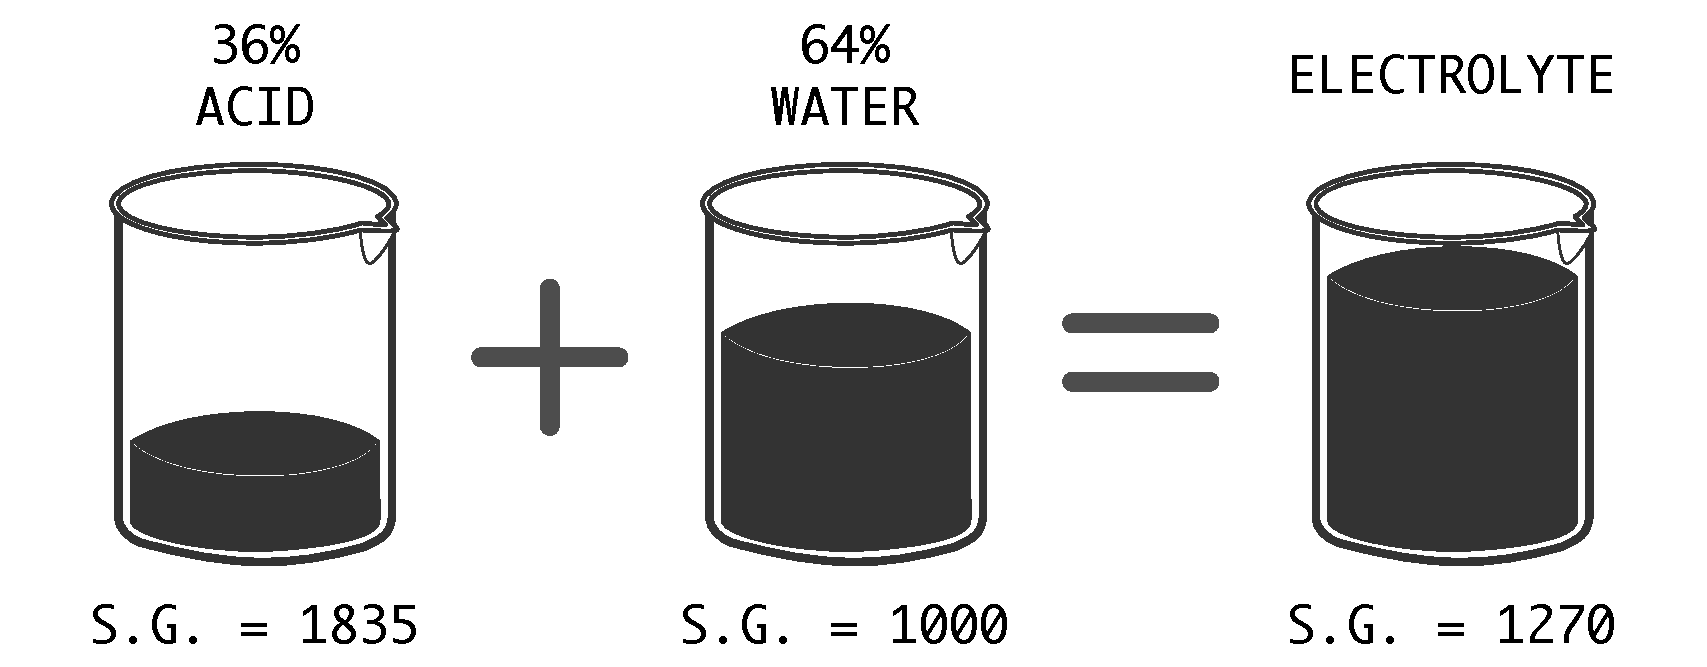
\includegraphics[width=0.7\linewidth]{./Resources/Images/Specific_Gravity.pdf}
  \end{center}

  \vspace{-10pt}  
  \begin{itemize}
    \item Sulphuric Acid ($H_{2}SO_{4}$) is used as the electrolyte for automotive batteries.
    \item ($H_{2}SO_{4}$) \textbf{\textit{Specific Gravity}} ranging from 1220 to 1280 is employed.
    \item Its concentration decides the chemical action in the cell.
  \end{itemize}
\end{frame}

\begin{frame}    %----SLIDE
  \frametitle{Battery Case}
  \fontsize{7pt}{10}\selectfont
  
  \begin{center}
    Battery case holds the electrolyte and the individual battery cells. 
  \end{center}
  
  \begin{itemize}
    \item The plates are raised up off the bottom of the case with ribs to prevent them from shorting out if any of the active materials (lead, etc.) should happen to fall from the plates.
    \item Usually made of polypropylene, hard rubber, plastic base materials.
    \item Translucent plastic cases allow checking electrolyte level without removing the vent caps - usually marked with upper \& lower electrolyte level.
  \end{itemize}
  
  \begin{center}
    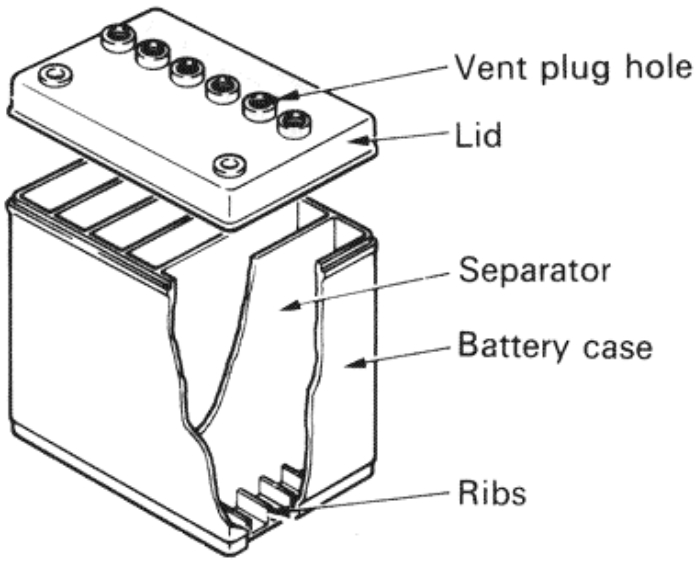
\includegraphics[width=0.5\linewidth]{./Resources/Images/battery_case.jpg}
  \end{center}
  
\end{frame}

\begin{frame}    %----SLIDE
  \frametitle{Vent Plugs}
  \fontsize{7pt}{10}\selectfont
  
  \begin{center}
    Vent plugs primarily cover the holes that are used for adding electrolyte.
  \end{center}
  
  \begin{itemize}
    \item Designed to separate the $H_{2}SO_{4}$ mist \& the $H_{2}$ gas that forms when the battery charges.
    \item Condenses $H_{2}SO_{4}$ mist and drop back into the battery, allowing $H_{2}$ gas to escape through the vent holes to the atmosphere.
    \item Translucent plastic cases allow checking electrolyte level without removing the vent caps - usually marked with upper \& lower electrolyte level.
  \end{itemize}
  
  \begin{center}
    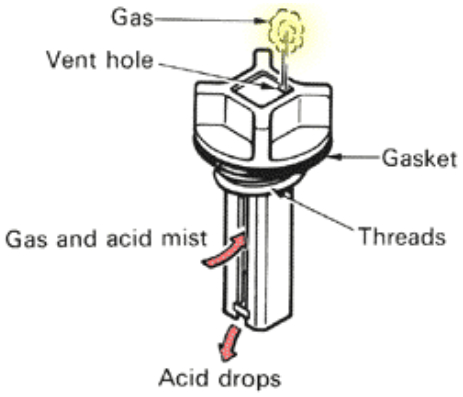
\includegraphics[width=0.4\linewidth]{./Resources/Images/vent_plug.jpg}
  \end{center}
  
\end{frame}

\begin{frame}    %----SLIDE
  \frametitle{Other Parts}
  \fontsize{10pt}{16}\selectfont

  \textbf{Cell Connectors:}  
  \begin{itemize}
    \item They provide electrical connection between the Cells of the battery.
    \item After assembling the cells in the case, they are burned to the strap posts.
  \end{itemize}
  
  \textbf{Battery Terminal:}
  \begin{itemize}
    \item Helps forming a connection to the automobile electrical circuit.
    \item Cables could be detachable using bolts or directly soldered to the terminal.
  \end{itemize}
  
  \textbf{Battery Cover \& Jars:}
  \begin{itemize}
    \item Cover facilitates the escape of gas during charge.
    \item Cover provides space for expansion of electrolyte when heated.
  \end{itemize}
\end{frame}


\begin{frame}    %----SLIDE
  \frametitle{Exploded View Example ...}  
  \begin{figure}
    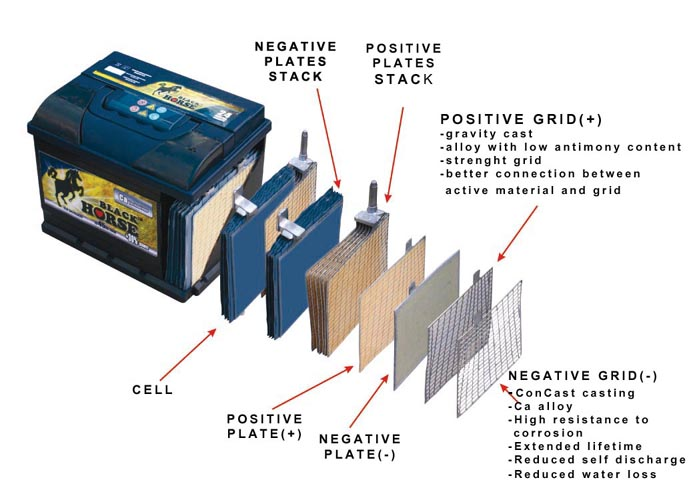
\includegraphics[width=0.9\linewidth]{./Resources/Images/exploded_view.jpg}
  \end{figure}
\end{frame}




%------------------------------------------------
\section{Chemical Action}
%------------------------------------------------

{ % all template changes are local to this group.
    \setbeamertemplate{navigation symbols}{}
    \begin{frame}[plain]
        \begin{tikzpicture}[remember picture,overlay]
            \node[at=(current page.center)] {
                
\includegraphics[width=\paperwidth]{./Resources/Images/Chemical_Action.pdf}
            };
        \end{tikzpicture}
     \end{frame}
}

\subsection{During Charging}

\begin{frame}    %----SLIDE
  \frametitle{Chemical Action During Charge}
  \begin{figure}
    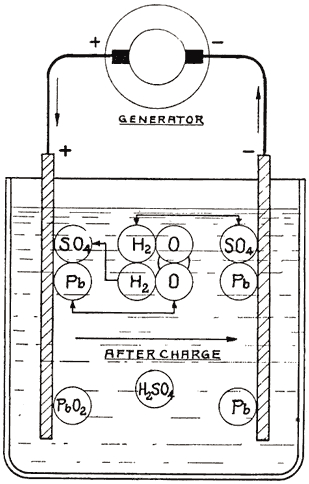
\includegraphics[width=0.4\linewidth]{./Resources/Images/chemistry_during_charge.jpg}
  \end{figure}
\end{frame}

\begin{frame}    %----SLIDE
  \frametitle{Chemical Action During Charge ...}
  \fontsize{8pt}{12}\selectfont
    
  \textbf{At +Ve Plate:}
  \begin{center}
    $ PbSO_{4} + 2H_{2}O \rightleftharpoons PbO_{2} + H_{2}SO_{4} + H_{2} \uparrow$
  \end{center}
  \textbf{At -Ve Plate:}
  \begin{center}
    $ PbSO_{4} + H_{2}O \rightleftharpoons Pb + H_{2}SO_{4} + O \uparrow$
  \end{center}  
  \textbf{Entire Charging Action:}
  \begin{center}
    $ 2PbSO_{4} + 2H_{2}O \rightleftharpoons PbO_{2} + Pb + 2H_{2}SO_{4} $
  \end{center}  


On continuous charging $H_{2}$ and $O_{2}$ rise to the surface of the electrolyte and escape from the cell. 
This is defined as \textbf{\textit{gassing}}, which is an indication of the cell is fully charged. \textbf{During Charge,
acid is driven out of the plates.}
\end{frame}

\subsection{During Discharging}

\begin{frame}    %----SLIDE
  \frametitle{Chemical Action During Discharge}
  \begin{figure}
    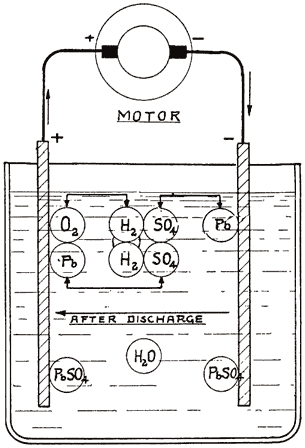
\includegraphics[width=0.4\linewidth]{./Resources/Images/chemistry_during_discharge.jpg}
  \end{figure}
\end{frame}

\begin{frame}    %----SLIDE
  \frametitle{Chemical Action During Discharge ...}
  \fontsize{8pt}{12}\selectfont
    
  \textbf{At +Ve Plate:}
  \begin{center}
    $ PbO_{2} + H_{2}SO_{4} \rightleftharpoons PbSO_{4} + H_{2}O + O \uparrow$
  \end{center}
  \textbf{At -Ve Plate:}
  \begin{center}
    $ Pb + H_{2}SO_{4} \rightleftharpoons PbSO_{4} + H_{2} \uparrow$
  \end{center}  
  \textbf{Entire Charging Action:}
  \begin{center}
    $ PbO_{2} + Pb + 2H_{2}SO_{4} \rightleftharpoons 2PbSO_{4} + 2H_{2}O $
  \end{center}  


Chemically discharging consists of changing the spongy lead and lead peroxide into lead sulphate 
and the abstraction of the acid from the electrolyte. \textbf{During discharge the acid goes into the plates.}
\end{frame}



%------------------------------------------------
\section{Electrical Action}
%------------------------------------------------

{ % all template changes are local to this group.
    \setbeamertemplate{navigation symbols}{}
    \begin{frame}[plain]
        \begin{tikzpicture}[remember picture,overlay]
            \node[at=(current page.center)] {
                
\includegraphics[width=\paperwidth]{./Resources/Images/Electrical_Action.pdf}
            };
        \end{tikzpicture}
     \end{frame}
}

 \begin{frame}   %----SLIDE
    \frametitle{Interaction}
    \fontsize{9pt}{14}\selectfont
    
    \bigskip
    Considered electrically, the changes are more complex. The following parameters and interaction between them must be considered:
    \bigskip
    
    \begin{itemize}
      \item Voltage
      \item Internal resistance
      \item Rate of discharge
      \item Capacity
    \end{itemize}
  \end{frame}

\subsection{During Charging}

  \begin{frame}    %----SLIDE
    \frametitle{Electrical Action During Charge}
    \begin{figure}
      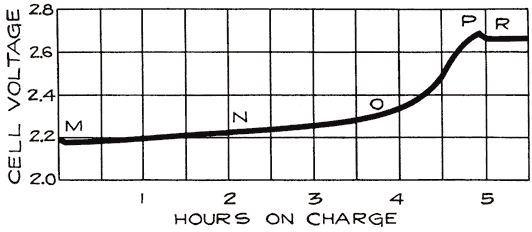
\includegraphics[width=0.8\linewidth]{./Resources/Images/voltage_during_charge.jpg}
    \end{figure}
    Voltage rises rapidly for a fraction of the first minute of the charge, \& drops rapidly
    to a normal value and thereafter begins to raise steadily to the end of the charge.
  \end{frame}

  \begin{frame}    %----SLIDE
  \frametitle{Process...}
  \fontsize{9pt}{14}\selectfont
    \vspace{-20pt}
    \begin{figure}
      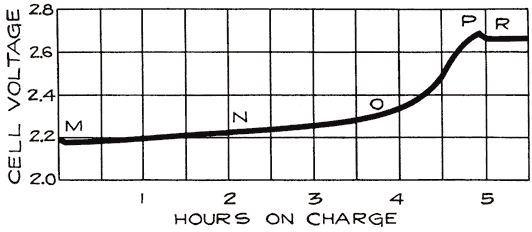
\includegraphics[width=0.6\linewidth]{./Resources/Images/voltage_during_charge.jpg}
    \end{figure}

    \begin{itemize}
      \item At point \textbf{O} the voltage begins to rise very rapidly due to the $PbSO_{4}$ in the plate decreasing. Bubbles of gas rises throughout the electrolyte.
      \item At point \textbf{P} the last portion of $PbSO_{4}$ are removed and acid is no longer formed. $H_{2}$ \& $O_{2}$ gases are formed rapidly.
      \item Voltage becomes constant at \textbf{R} $\approx$ 15 to 16 Volts.
    \end{itemize}    
  \end{frame}
  
  \begin{frame}   %----SLIDE
  \frametitle{Density}
    \begin{center}
      Progress of the Charge is generally determined the density/Specific Gravity of the electrolye in the range 1220 to 1280 measured at 23\textcelsius.
    \end{center}
  \end{frame}


\subsection{During Discharging}

  \begin{frame}    %----SLIDE
    \frametitle{Electrical Action During Discharge}
    \begin{figure}
      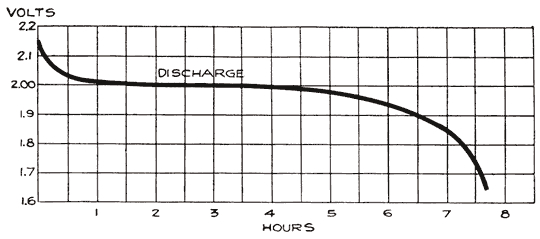
\includegraphics[width=0.8\linewidth]{./Resources/Images/voltage_during_discharge.jpg}
    \end{figure}
    As soon as charging circuit is opened the cell voltage drops rapidly to about 2.1V, within
    3 or 4 minutes due to the formation of thick layer of $PbSO_{4}$ on the surface of -Ve plate
    \& between lead peroxide and the metal of the +Ve plate.
  \end{frame}

  \begin{frame}    %----SLIDE
  \frametitle{Process...}
  \fontsize{9pt}{14}\selectfont
    \vspace{-20pt}
    \begin{figure}
      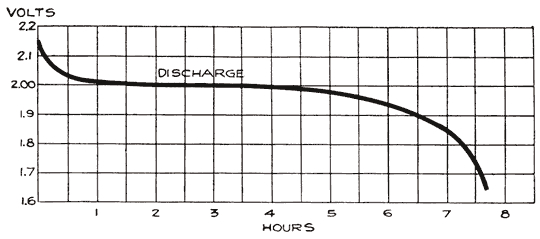
\includegraphics[width=0.7\linewidth]{./Resources/Images/voltage_during_discharge.jpg}
    \end{figure}
    \vspace{-20pt}
    
    \begin{itemize}
      \item When current is being drawn from the battery the sudden drop is due to the \textbf{internal resistance of the cell},
      formation of more sulphate and the abstraction of the acid from the electrolyte which fills the pores of the plate.
      \item The limiting value of 1.75V/cell applies to a continuous discharge at a moderate rate. During cranking it may be 
      permitted to a lesser voltage.
      \item Voltage does not depend upon the area of the plate surface but upon the nature of active material and electrolyte.
    \end{itemize}    
  \end{frame}

  \begin{frame}   %----SLIDE
  \frametitle{Density}
    \vspace{-10pt}
    \begin{center}
      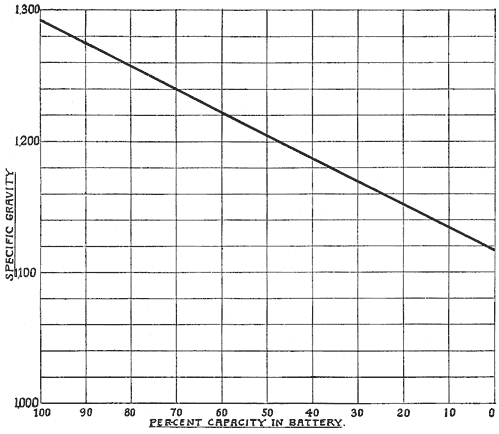
\includegraphics[width=0.5\linewidth]{./Resources/Images/density_during_discharge.jpg}
    \end{center}
    The discharge process may be continued upto a Specific Gravity of 1150 at normal temperature due to the fact that
    further discharge will reduce the life of the battery and battery capacity cannot be expected below 1150 as shown above.
  \end{frame}
  
  

%------------------------------------------------
\section{Battery Capacity}
%------------------------------------------------

\begin{frame}     %----SLIDE
  \frametitle{Capacity of automotive battery}
  \fontsize{9pt}{14}\selectfont
  
  \textbf{What is it ?}
  \begin{itemize}
    \item Capacity is the product of Current(\textbf{\textit{I}}) drawn from the battery \& no. of Hours(\textbf{\textit{T}}) the current flows, measued in \textbf{Ampere Hour.}
    \item Leading health indicator of a battery.
  \end{itemize}
  
  \textbf{Limit:}
  \begin{itemize}
    \item In practice we do not discharge the battery to a voltage less than 1.75V/cell, except when the rate of discharge is high, like during cranking.
  \end{itemize}
  
  \textbf{So ?}
  \begin{itemize}
    \item Thus capacity is measured by the no. of hours it can furnish before its voltage drops below 1.75V/cell.
  \end{itemize}  
\end{frame}

\begin{frame}     %----SLIDE
  \frametitle{Capacity Ratings}
  \fontsize{8pt}{14}\selectfont
  
  \textbf{What is it ?}: Several Battery capacity ratings have been established by Battery Council International (BCI) that helps to determine the current capacity of a battery.
  It is an indication of battery's ability to develop and deliver high amperage current to the starter and provide reserve power to the electrical system.
  
  \begin{itemize}
    \item \textbf{Cold Cranking Amps (CCA) rating:} Indicates the ability to deliver specified current @ low temperatures - of a fully charged battery 
    for 30 sec. @ 0degF (-17.8\textcelsius) with terminal voltage not less than 7.2V.
    \item \textbf{Cranking Amps (CA) rating:} Indicates the ability to deliver a cranking current at 32degF.
    \item \textbf{Reserve Capacity rating:} It is the time in minutes a vehicle can be driven \textbf{after the charging system fails}. It is the length of time a fully
    charged battery can supply 25A, before the terminal voltage falls below 10.5V @ 26.7\textcelsius.
    \item \textbf{Ampere Hour rating:} It is the amount of current a fully charged battery could supply for 20 hrs. without having the terminal voltage below 10.5V, @ 26.7\textcelsius.
  \end{itemize}
  
\end{frame}

\begin{frame}     %----SLIDE
  \frametitle{Capacity Factors ...}
  \fontsize{9pt}{14}\selectfont
  
  \textbf{Based on Design \& Construction:}
  \begin{itemize}
    \item Area of plate surface.
    \item Quantity, arrangement \& porosity of active material.
    \item Quantity \& Strength of electrolyte.
    \item Circulation of electrolyte.
  \end{itemize}

  \bigskip
  \textbf{Based on Conditions of Operation:}
  \begin{itemize}
    \item Rate of discharge
    \item Temperature
  \end{itemize}  
\end{frame}



%------------------------------------------------
\section{Internal Resistance}
%------------------------------------------------

\begin{frame}     %----SLIDE
  \frametitle{Internal Resistance of automotive battery}
  \fontsize{9pt}{14}\selectfont
  
  \textbf{What is it ?}
  \begin{itemize}
    \item Resistance offered by the battery to the low of the current through it results in a loss of voltage \& heating. Usually it is measured about
    0.05$\Omega$, between the terminals of the cell/battery.
  \end{itemize}
  
  \textbf{Why is it there ?}
  \begin{itemize}
    \item Due to grids including terminals, connecting links \& framework upon which active materials are paster, that vary as the temperature of the grid varies.
    \item Electrolyte - main cause of internal resistance, can be reduced to optimum value by maintaining the Specific Gravity of 1150 to 1280.
    \item Active material - includes its own resistance \& electrolyte in the pores of the active material that varies during charging and discharging.
  \end{itemize} 
\end{frame}

\begin{frame}     %----SLIDE
  \frametitle{Internal Resistance \& Specific Gravity of Electrolyte}
  
  \begin{figure}
    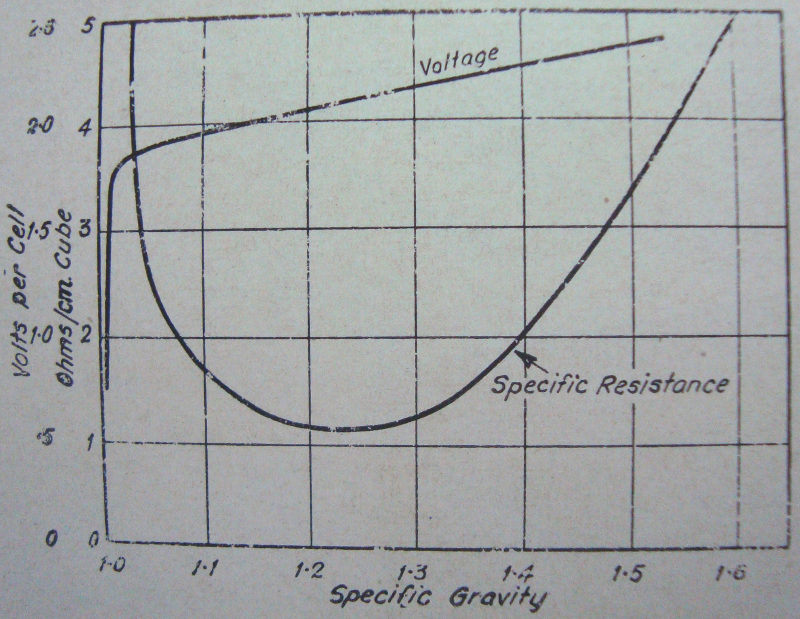
\includegraphics[width=0.8\linewidth]{./Resources/Images/specific_gravity_specific_resistance.png}
  \end{figure}
\end{frame}

\begin{frame}     %----SLIDE
  \frametitle{Internal Resistance during Charging \& Discharging}
  
  \begin{figure}
    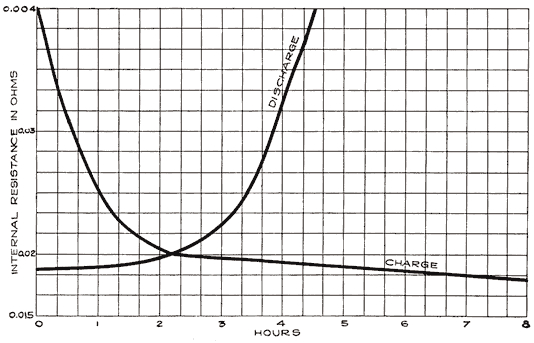
\includegraphics[width=0.8\linewidth]{./Resources/Images/internalresistance_charge_discharge.jpg}
  \end{figure}
\end{frame}


%------------------------------------------------
\section{Electrical Equivalent}
%------------------------------------------------


\begin{frame}[label=electrical_equivalent]    %----SLIDE
  \frametitle{Electrical equivalent of the Electrochemical phenomemena}
  \fontsize{8pt}{10}\selectfont
    \vspace{-10pt}
    \begin{figure}
      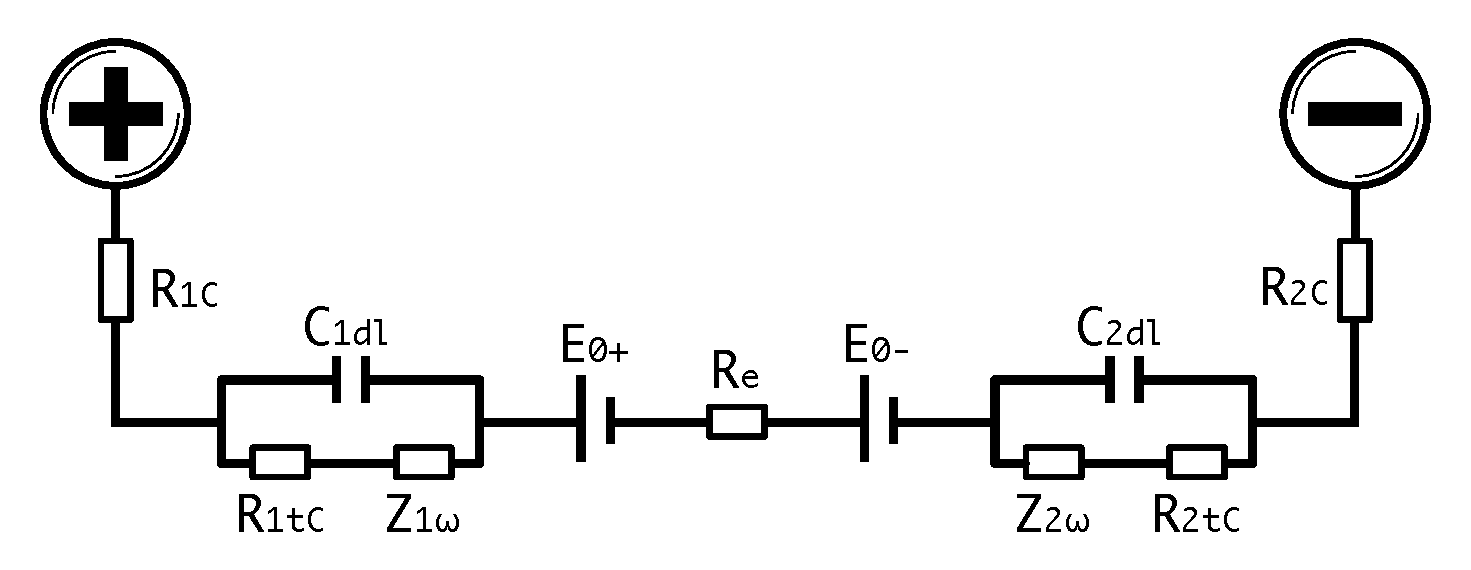
\includegraphics[width=0.5\linewidth]{./Resources/Images/Electrical_Equivalent.pdf}
    \end{figure}
    \vspace{-10pt}
   
      The total equilibrium potential of the battery is the difference between the potentials of the two electrodes:
      \vspace{-8pt}
      \begin{center}
        $E_{eq} = E_{0+} - E_{0-}$
      \end{center}
      \vspace{-5pt}
      
      Internal resistance of the battery results in the sum of various connector resistances \& electrolyte resistance: \\
      \vspace{-8pt}
      \begin{center}
        $R_{\omega} = R_{1c} + R_{2c} + R_{e}$
      \end{center}
      \vspace{-5pt}
      
      $C_{1dl}$ \& $C_{2dl}$ represent the double layer capacitane on each electrode, caused by the charge distribution between the electrode \& electrolyte.
      
      \medskip
      $R_{1tc} \& R_{2tc}$ represents the phenomenon of chage transfer resistance between the electrode and electrolyte. This causes an over voltage of charge transfer $\eta_{tc}$.\\

      \medskip
      $Z_{1\omega} \& Z_{2\omega}$ represents the phenomenon of diffusion, caused by grade of concentration of electrolyte near electrode. It again causes a second over voltage of
      concentration $\eta_{diff}$. This is called as \href{https://en.wikipedia.org/wiki/Warburg_element}{\textbf{\textit{\underline{warburg impedance}}}}.
      
      \begin{center}
        \hyperlink{analysis}{\beamergotobutton{Goto Analysis}}  
      \end{center}
      
\end{frame}



%------------------------------------------------
\section{Automotive Battery Care}
%------------------------------------------------

{ % all template changes are local to this group.
    \setbeamertemplate{navigation symbols}{}
    \begin{frame}[plain]
        \begin{tikzpicture}[remember picture,overlay]
            \node[at=(current page.center)] {
                
\includegraphics[width=\paperwidth]{./Resources/Images/Battery_Care.pdf}
            };
        \end{tikzpicture}
     \end{frame}
}

\begin{frame}     %----SLIDE
  \frametitle{Battery Care in Vehicles}
  \fontsize{8pt}{14}\selectfont
  \textbf{In General:}
  \begin{itemize}
    \item Keep interior of battery box clean \& dry.
    \item Put nothing but battery in battery box.
    \item Keep battery clean and dry to avoid leakage of current.
    \item Firm fixation.
    \item Sufficient slack in cables connected to the battery.
    \item Inspect the battery twice a month in winter \& every week in summer.
  \end{itemize}
\end{frame}

\begin{frame}     %----SLIDE
  \frametitle{Battery Care in Vehicles ...}
  \fontsize{8pt}{14}\selectfont  
  
  \textbf{Specific Gravity:}
  \begin{itemize}
    \item Specific Gravity (Sp.gr.) of the electrolyte measured periodically are recorded permanently for future reference.
    \item Electrolyte must not spill over while testing the electrolyte.
    \item Electrolyte must be retured to same cell during testing.
    \item Sp.gr. of all cells should rise and fall together.
    \item If Sp.gr of one cell is lower than the other cells in series, it has internal trouble(may be short circuit).
    \item If entire battery shows a Sp.gr below 1200, then the battery is not receiving enough charge.
  \end{itemize}
  
  \textbf{During Idle/Not in Use:}
  \begin{itemize}
    \item Filled with distilled water \& given a complete charge.
    \item After every 6 to 8 weeks, battery is given a freshening charge without rising the temperature.
  \end{itemize}
\end{frame}


\subsection{Troubles}               %----SUBSECTION

{ % all template changes are local to this group.
    \setbeamertemplate{navigation symbols}{}
    \begin{frame}[plain]
        \begin{tikzpicture}[remember picture,overlay]
            \node[at=(current page.center)] {
                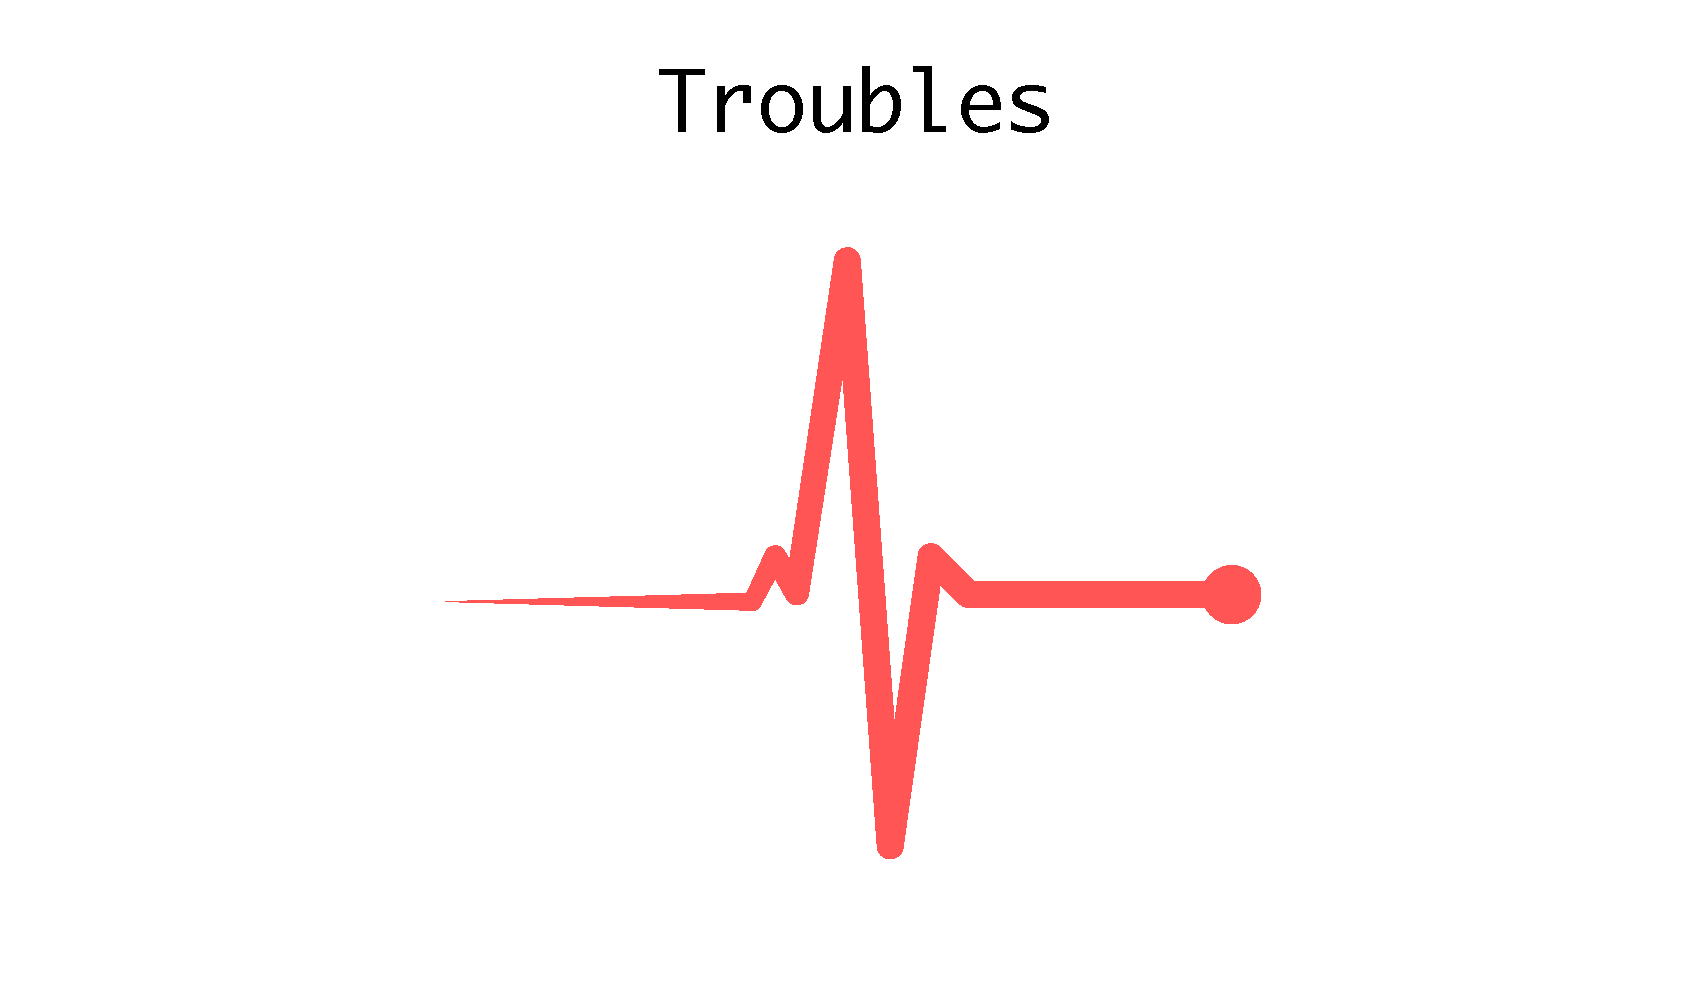
\includegraphics[width=\paperwidth]{./Resources/Images/Troubles.pdf}
            };
        \end{tikzpicture}
     \end{frame}
}

\begin{frame}     %----SLIDE
  \frametitle{What are the Troubles ?}
  \fontsize{8pt}{14}\selectfont
  \begin{center}
    When there is slackness in caring the battery, it becomes subjective to a number of \textbf{\textit{preventable}} diseases
    that leads to inefficiency. \\
    - - - - - - \\
    Most battery diseases are contagious and if one part fails, \\ eventually other related parts also affected.
  \end{center}
  
  \textbf{Major troubles are with:}
  \begin{itemize}
    \item Plates
    \item Separators
    \item Jars
    \item Container
    \item Cell connectors \& Terminals
    \item Electrolyte
  \end{itemize}
\end{frame}

\begin{frame}     %----SLIDE
  \frametitle{Plate Troubles}
  \fontsize{8pt}{14}\selectfont
  \begin{center}
    Plates are the \textbf{\textit{vitals}} of the battery that affect life of the battery than other parts.
    They are also very difficult to diagonise the troubles associated.
  \end{center}
  
  \textbf{Sulphation:} Formation of lead sulphate ($PbSO_{4}$) on plates.
  \begin{itemize}
    \item Over discharge
    \item Keeping idle
    \item Starvation
    \item Electrolyte below the top of plates
    \item Impurities
    \item Adding acid instead of distilled water
    \item Over heating
  \end{itemize}
\end{frame}

{ % all template changes are local to this group.
    \setbeamertemplate{navigation symbols}{}
    \begin{frame}[plain]
        \begin{tikzpicture}[remember picture,overlay]
            \node[at=(current page.center)] {
                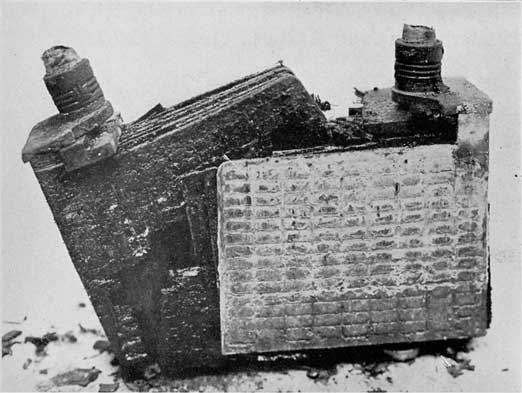
\includegraphics[width=0.7\paperwidth]{./Resources/Images/sulphation.jpg}
            };
        \end{tikzpicture}
     \end{frame}
}

\begin{frame}     %----SLIDE
  \fontsize{8pt}{14}\selectfont
  
  \textbf{Buckling:} Bending \& Twisting of plates due to unequal expansion of different parts of the plates due to:
  \begin{itemize}
    \item Over discharge
    \item Continued operation in discharged condition
    \item Charging at high rates
    \item Non-Uniform distribution of currents over the plates
    \item Defective grid alloy
  \end{itemize}
  
  \begin{center}
    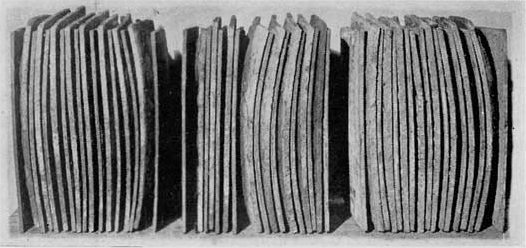
\includegraphics[width=0.8\linewidth]{./Resources/Images/buckling.jpg}
  \end{center}
\end{frame}

\begin{frame}     %----SLIDE
  \fontsize{8pt}{14}\selectfont
  
  \textbf{Shedding/Loss of Active Material:} Loosening of lead peroxide of +ve plate which reduces the capacity of the plates due to:
  \begin{itemize}
    \item Normal Shedding
    \item Over charging/Excessive charging rate
    \item Charging sulphated plates at too high rate
    \item Charging only \textbf{part} of the plate
    \item Freezing
  \end{itemize}
  
  \begin{center}
    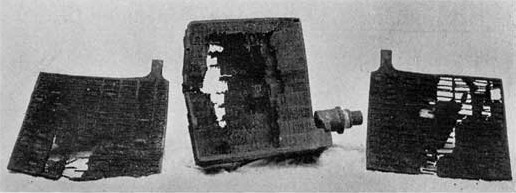
\includegraphics[width=0.8\linewidth]{./Resources/Images/shedding.jpg}
  \end{center}
\end{frame}

\begin{frame}     %----SLIDE
  \fontsize{8pt}{14}\selectfont
  
  \textbf{Loose Active Material:} Active material are no longer in contact with the grid, may be one of the cause of chemical action
  on grids shifted from active material to the grid itself, due to:
  \begin{itemize}
    \item Over discharge
    \item Buckling
  \end{itemize}

  \textbf{Impurities:} 
  \begin{itemize}
    \item That attack the plates due to the acids other than $H_{2}SO_{4}$ which dissolve the lead grids -- disintegrating plates into pieces.
    \item That do not attack grid/separators, but cause internal self discharge due to methods other than lead causing hydrogen bubbles 
    giving electrolyte a milky appearance.
  \end{itemize}  
  
  \textbf{Corroded grids:} Thin, weak \& corroded due to the chemical action of electrolyte over the grid
  \begin{itemize}
    \item Impurities other than $H_{2}SO_{4}$
    \item High temperature
    \item Aging
  \end{itemize}
\end{frame}

\begin{frame}     %----SLIDE
  \frametitle{Separator Troubles}
  \fontsize{8pt}{14}\selectfont
  \begin{center}
    Separators are the weakest part, performing important duty for the battery.
  \end{center}
  
  Troubles are:
  \begin{itemize}
    \item Not properly expanded before installation.
    \item Improper inspection (cracked separator).
    \item \textbf{\textit{Treeing}} between plates, causing short circuit.
    \item Improperly treated separators will cause battery to show low voltage at high rates of discharge, particularly in cold weather.
    \item Rotted/Carbonized, due to overage, over heating or high gravity electrolyte.
    \item Pores clogged due to dust, impurities from impure water \& $PbSO_{4}$.
    \item Edges chiseled off -- buckling plate cut through lower edges of separator.
  \end{itemize}
\end{frame}

\begin{frame}     %----SLIDE
  \frametitle{Container Troubles}
  \fontsize{8pt}{14}\selectfont
  \begin{center}
    Eventhough modern day batteries are made with polypropylene/high grade components, to reduce the weight, still troubles occur due to:
  \end{center}
  
  \begin{itemize}
    \item Rough handling.
    \item Battery not properly fitted.
    \item Any weight placed on top of the battery.
    \item Freezing.
    \item Defective Jars.
    \item Expansion in cell.
  \end{itemize}
\end{frame}

\begin{frame}     %----SLIDE
  \frametitle{Cell Connectors \& Terminal Troubles}
  \fontsize{8pt}{14}\selectfont
  \begin{center}
    This is a common trouble which should be guarded very carefully.
  \end{center}
  
  \textbf{Corrosion:} Indicated by the presence of greenish substance on the battery terminals (especially +ve) due to:
  \begin{itemize}
    \item Too much water added to cells.
    \item Battery not fastened firmly.
    \item Battery poorly sealed.
    \item Vent cap loose.
    \item Electrolyte spilled on top of cover while measuring Sp.gr.
    \item Battery cables damaged or loose.
    \item Attaching bare wires on battery terminals.
    \item Loose connections in the terminals.
  \end{itemize}
\end{frame}

\begin{frame}     %----SLIDE
  \frametitle{Electrolyte Troubles}
  \fontsize{8pt}{14}\selectfont

  \begin{itemize}
    \item Low gravity due to addition of distilled water.
    \item High gravity due to addition of acid instead of distilled water.
    \item Low level due to improper topup maintenance of battery.
    \item No rise in Sp.gr. due to plates not taking full charge or water is used to replace the spilled electrolyte.
    \item \textbf{Stratification} of electrolyte due to starvation of charge.
    \item \textbf{Milky electrolyte:} mixing of $PbSO_{4}$ in battery acid or gassing or impurities.
  \end{itemize}
\end{frame}

\begin{frame}     %----SLIDE
  \frametitle{Other General Troubles ...}
  \fontsize{8pt}{12}\selectfont
  
  \textbf{Open Circuit:}
  \begin{itemize}
    \item Poor burning of connectors to posts.
    \item Terminals broken off.
    \item Acid on soldered joints.
    \item Defective posts.
    \item Plates improperly burned.
  \end{itemize}
  
  \textbf{Battery Discharged:}
  \begin{itemize}
    \item Due to excessive use of starting motor.
    \item Failure of generator.
    \item Defective switches.
    \item Defective regulator.
    \item Addition of accessories or use of too large lamps.
    \item Defective wiring.
    \item Insufficient charging rates.
    \item Batteries allowed to remain idle.
  \end{itemize}
\end{frame}

\begin{frame}     %----SLIDE
  \fontsize{8pt}{12}\selectfont
  
  \textbf{Dead cells:}
  \begin{itemize}
    \item Worn out separators.
    \item Foreign material.
    \item Accumulation of sediments.
    \item Badly sulphated plates \& separators.
    \item Impurities which attack the plates.
  \end{itemize}
  
  \textbf{Loss of capacity:}
  \begin{itemize}
    \item Impurities in the electrolyte.
    \item Sulphation.
    \item Loose active material.
    \item Incorrect Sp.gr. of electrolyte.
    \item Separators clogged.
    \item Shedding.
    \item Low level of electrolyte.
    \item Reversal of plates.
    \item Effect of age.
  \end{itemize}
\end{frame}



%------------------------------------------------
\section{Analysis of Degradation}
%------------------------------------------------

{ % all template changes are local to this group.
    \setbeamertemplate{navigation symbols}{}
    \begin{frame}[plain]
        \begin{tikzpicture}[remember picture,overlay]
            \node[at=(current page.center)] {
                
\includegraphics[width=\paperwidth]{./Resources/Images/Analysis_Degradation.pdf}
            };
        \end{tikzpicture}
     \end{frame}
}

\begin{frame}     %----SLIDE
  \frametitle{Analysis Tools:}
  \fontsize{10pt}{16}\selectfont
  
  Tools such as \href{http://www.journal.esrgroups.org/jes/papers/4_2_2.pdf}{\textbf{\underline{causal tree and fault tree analysis}}} offer an inductive \& deductive analysis to evaluate safety \& reliability of a complex system such as lead acid battery.\\
  
  \bigskip
  The analysis of the causality chain of lead-acid battery is based on two stages:
  
  \begin{itemize}
    \item 1st stage interested in development of causal tree presenting possible combination of events generated by \textbf{physicochemical} phenomena.
    \item 2nd stage completes causality chain with fault tree analysis(FTA) with \textbf{electrical equivalent circuit} \& experimental determination of \textbf{parameters} in the 
    circuit, according to each mode of degradation.
  \end{itemize}
  
\end{frame}

\begin{frame}     %----SLIDE
  \frametitle{What Causes Degradation ?}
  \fontsize{8pt}{12}\selectfont
  
  The aging mechanisms of batteries are the actual chemical \& mechanical events that cause its degradation, depending on the condition which it is operated. All the types of lead acid
  batteries suffer from same damage mechanisms but with different degrees.
  
  \bigskip
  \bigskip
  \textbf{Major aging process are:}
  \begin{itemize}
    \item Stratification of electrolyte.
    \item Sulfating of the electrodes.
    \item Corrosion of the electrodes.
    \item Non cohesion of the active mass.
  \end{itemize}
  
\end{frame}


\subsection{Causal Tree Analysis}          %----SUBSECTION

\begin{frame}     %----SLIDE
  \frametitle{Causality - Stratification of Electrolyte}
  \fontsize{8pt}{12}\selectfont
  \vspace{-10pt}
  Battery tends to stratify if it did not recieve a complete charge or kept under weak charge. With such conditions, distribution of electrolyte is not uniform with charge \& discharge 
  cycles.
  \vspace{-10pt}
  \begin{center}
    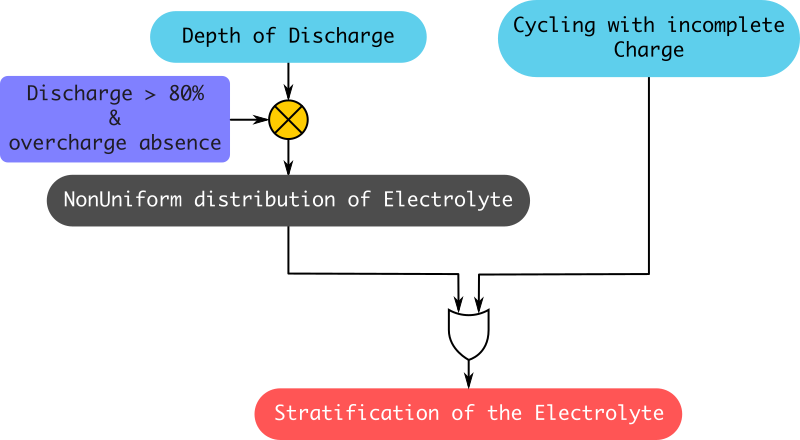
\includegraphics[width=0.8\linewidth]{./Resources/Images/analysis_causality_stratification.png}
  \end{center}
  \vspace{-10pt}
  The ions heavier than water tend to accumulate at the bottom of the battery, creating a \textbf{stratification of electrolyte}. Leads to reduced battery capacity by 
  concentrating chemical reaction to specific parts of electrodes.
\end{frame}

\begin{frame}     %----SLIDE
  \frametitle{Causality - Sulfating of Electrodes}
  \fontsize{8pt}{12}\selectfont
  When battery is discharged, sulfate cyrstals are formed at both the electrodes. When charged, the sulface crystals dissolve and form $PbO_{2}$ \& $Pb$ respectively on +ve and -ve 
  electrode respectively. If left at a low state of charge for longer period of time, sulfate crystals and do not dissolve easily when charged. This leads to hard or irreversible 
  \textbf{sulfating}.
  \vspace{-10pt}
  \begin{center}
    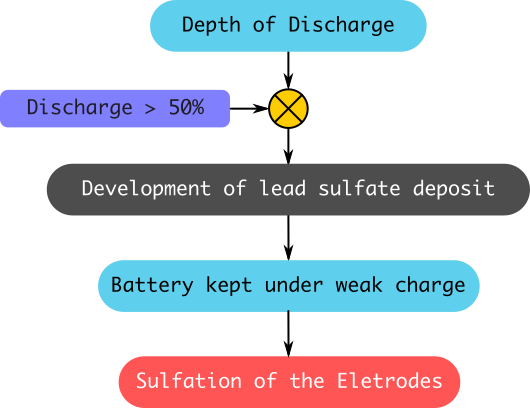
\includegraphics[width=0.5\linewidth]{./Resources/Images/analysis_causality_sulfation.png}
  \end{center}

  It creates an insulating layer that slows down the diffusion of the acid. Thus it is recommended not to discharge below 50\% and recharge back to 100\%.
\end{frame}

\begin{frame}     %----SLIDE
  \frametitle{Causality - Corrosion of Electrodes}
  \fontsize{8pt}{12}\selectfont
  \vspace{-8pt}
  Battery voltage, acid concentration and temperature are the three main factors that drive corrosion. Generally high voltage and increased concentration of acid increases the rate of 
  corrosion dramatically. Corrotion process is proportionately faster with rise in temperature.
  \vspace{-5pt}
  \begin{center}
    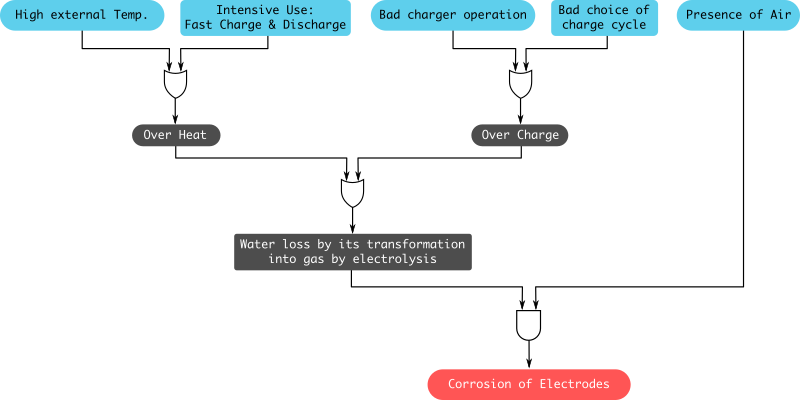
\includegraphics[width=0.9\linewidth]{./Resources/Images/analysis_causality_corrosion.png}
  \end{center}
  \vspace{-8pt}
  As part of grid corrodes, active mass has reduced the electrical conneciton to the terminals. Because of increase in corrosion layer, reduced conductivity, reduced cross section of 
  grid, internal resistance increases reducing the available capacity.
\end{frame}

\begin{frame}     %----SLIDE
  \frametitle{Causality - Non Cohesion of Active Mass}
  \fontsize{8pt}{12}\selectfont
  \vspace{-20pt}
  Non cohesion of active material is usually caused by shedding. Enough shedded material at the bottom of the jar can cause an electrical short. 

  \begin{center}
    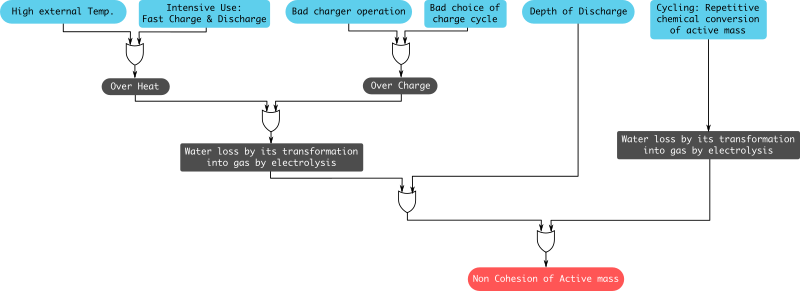
\includegraphics[width=\linewidth]{./Resources/Images/analysis_causality_lossofactivemass.png}
  \end{center}
  \vspace{-8pt}
  Gassing bubbles due to overcharging can also cause shedding. Depth of discharge and repetitive chemical transformation during charge \& discharge are responsible for non cohesion.
  Over time active mass on battery plates, degrades, changes structure - loosing some of electric transfer properties, reducing the capacity.
\end{frame}

\begin{frame}     %----SLIDE
  \frametitle{Overall Causality - Loss of Capacity}
  \begin{center}
    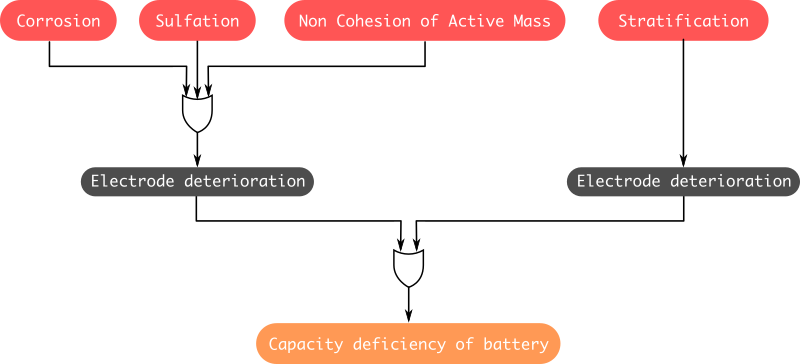
\includegraphics[width=\linewidth]{./Resources/Images/analysis_causality_overall.png}
  \end{center}
\end{frame}


\subsection{Fault Tree Analysis}          %----SUBSECTION

\begin{frame}[label=analysis]     %----SLIDE
  \frametitle{Fault Tree - from electrical equivalent}
  \fontsize{8pt}{10}\selectfont
  \begin{center}
    \hyperlink{electrical_equivalent}{\beamergotobutton{Goto Electrical Equivalent}}
  \end{center}
  \vspace{-8pt}
  \textbf{Fault tracing in Corrosion:}
  \vspace{-10pt}
  \begin{center}
    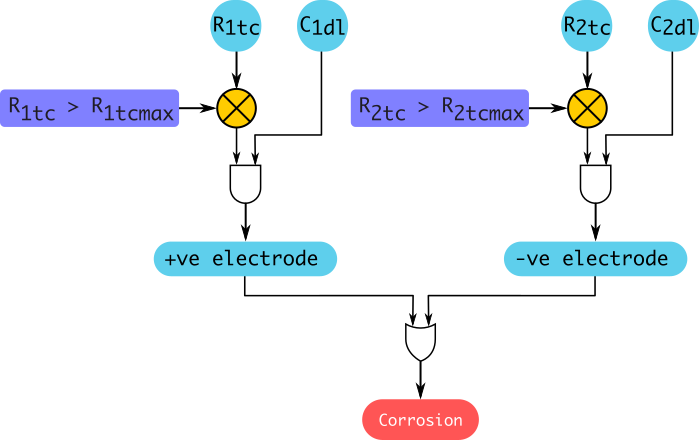
\includegraphics[width=0.55\linewidth]{./Resources/Images/analysis_faulttree_corrosion.png}
  \end{center}
  \vspace{-15pt}
  \textbf{Fault tracing in Sulfation:}
  \vspace{-10pt}  
  \begin{center}
    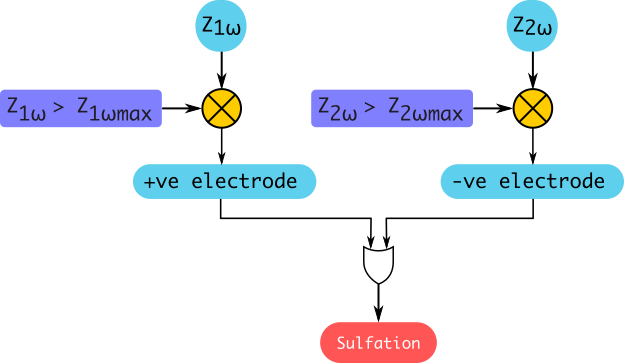
\includegraphics[width=0.55\linewidth]{./Resources/Images/analysis_faulttree_sulfation.png}
  \end{center}
\end{frame}

\begin{frame}     %----SLIDE
  \frametitle{Fault Tree - from electrical equivalent ...}
  \fontsize{8pt}{10}\selectfont
  \textbf{Fault tracing in Non cohesion of active mass:}
  \vspace{-5pt}
  \begin{center}
    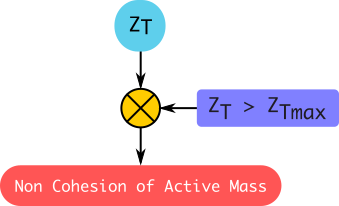
\includegraphics[width=0.4\linewidth]{./Resources/Images/analysis_faulttree_noncohesionactivemass.png}
  \end{center}
  \textbf{Fault tracing in Stratification:}
  \vspace{-10pt}  
  \begin{center}
    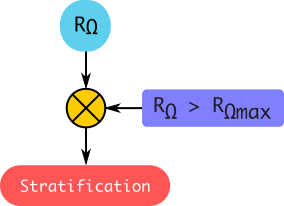
\includegraphics[width=0.35\linewidth]{./Resources/Images/analysis_faulttree_stratification.png}
  \end{center}
\end{frame}



%------------------------------------------------
\section{Instructions}
%------------------------------------------------

{ % all template changes are local to this group.
    \setbeamertemplate{navigation symbols}{}
    \begin{frame}[plain]
        \begin{tikzpicture}[remember picture,overlay]
            \node[at=(current page.center)] {
                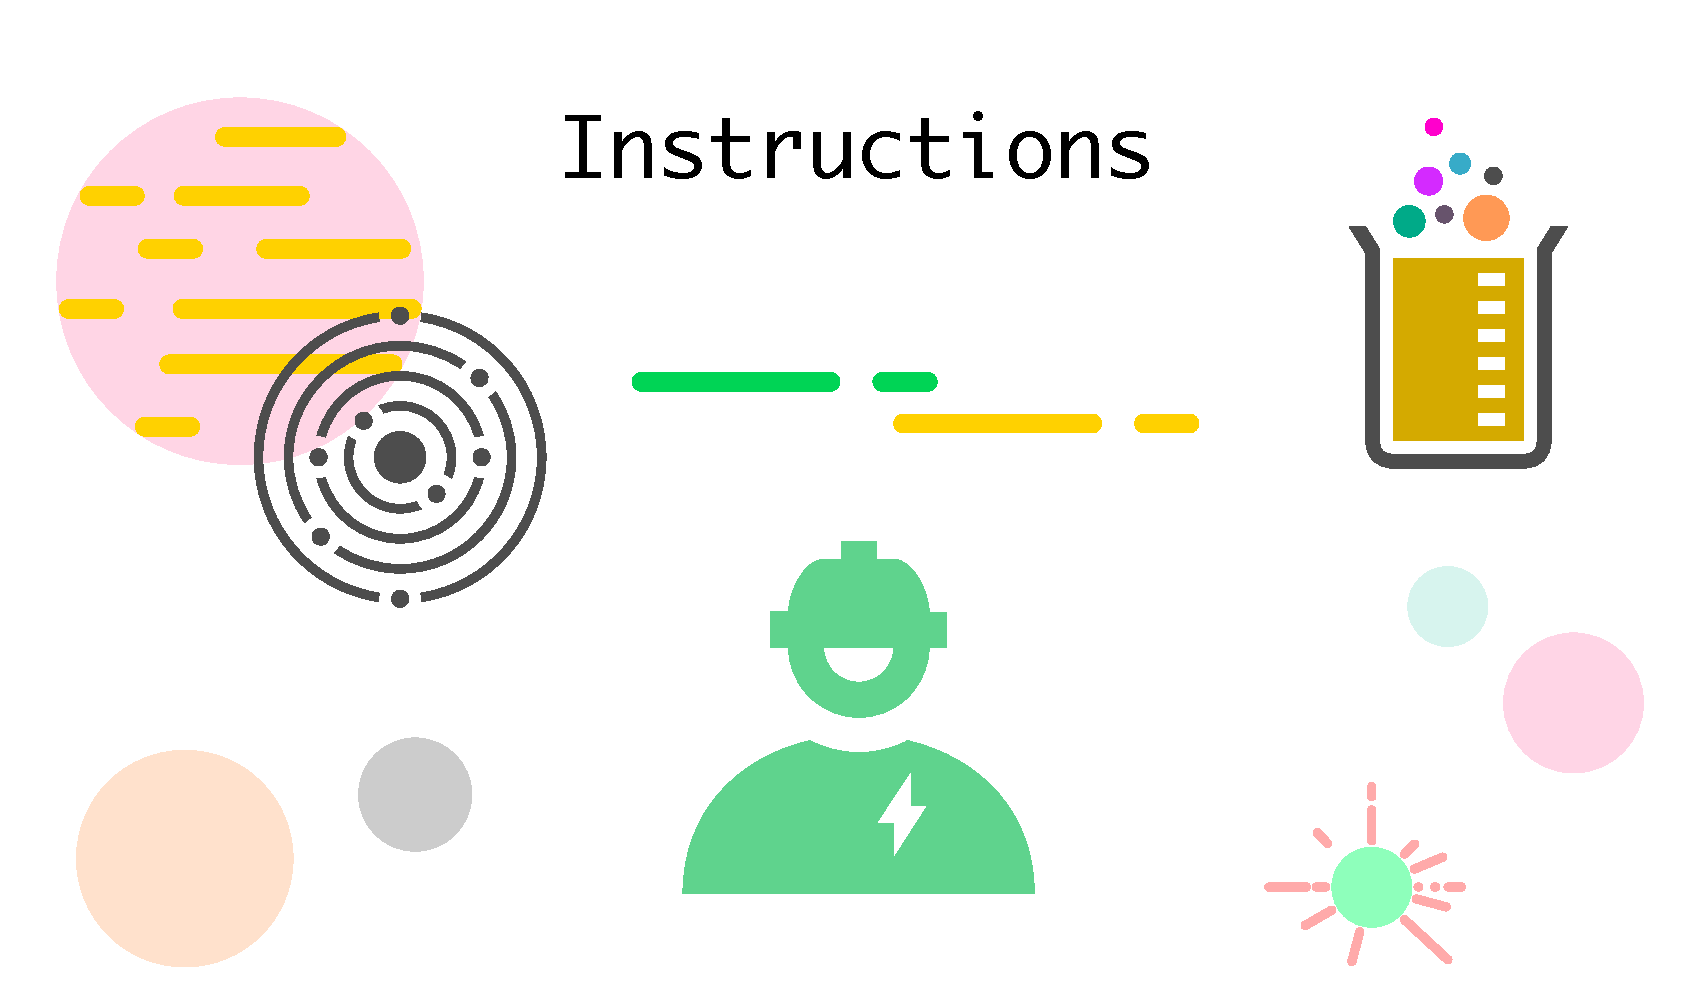
\includegraphics[width=\paperwidth]{./Resources/Images/Instructions.pdf}
            };
        \end{tikzpicture}
     \end{frame}
}

\subsection{Charging}         %----SUBSECTION

\begin{frame}     %----SLIDE
  \frametitle{Kind of Charging}
  \fontsize{7pt}{10}\selectfont
  \vspace{-8pt}
  \begin{itemize}
    \item Initial Filling \& Charging:
    \begin{itemize}
      \fontsize{7pt}{10}\selectfont
      \item @ 5\% of Ah for 48hrs.
      \item without rise in temperature.
      \item final consistent Voltage and Sp.Gr. for 5hrs without heavy gassing.
    \end{itemize}
    \item Bench Charging:
    \begin{itemize}
      \fontsize{7pt}{10}\selectfont
      \item @ 7.5\% of Ah.
      \item rating is reduced when battery is heavily sulfated.
    \end{itemize}
    \item Trickle Charging
    \item Regular Charging:
    \begin{itemize}
      \fontsize{7pt}{10}\selectfont
      \item for farm lighting or invertor batteries.
      \item to meet lighting and other demands.
    \end{itemize}
    \item Over Charging:
    \begin{itemize}
      \fontsize{7pt}{10}\selectfont
      \item extension of regular charging.
      \item once a month to prevent inequalities in cells.
    \end{itemize}
    \item Partial or Radid Charging:
    \begin{itemize}
      \fontsize{7pt}{12}\selectfont
      \item for farm lighting or invertor batteries, when there is not enough time for regular charging.
      \item @ double the charging rate until all cells are gassing, then reduce to normal rate.
    \end{itemize}    
  \end{itemize}
\end{frame}

\begin{frame}
  \frametitle{Rating \& Time for Charging}
  \fontsize{8pt}{11}\selectfont
  \textbf{Rating:}
  \begin{itemize}
    \item As long as excessive temp. \& too early gassing are avoided, any rate upto 7.5\% of Ah can be used.
    \item Temperature and Gassing must be watched carefully during charging.
    \item As a general rule, do not use rate higher than 10A, 5A is better (but takes more time).
    \item For heavily sulfated battery, less than 5A for days together would comeup.
  \end{itemize}
  
  \bigskip
  \textbf{Timing:}
  \begin{itemize}
    \item It is not determined by clock, but by cells, plates, electrolyte ...
    \item Continue charging until each cell is gassing freely (not violently), for 5hrs. after Sp.Gr. has stopped rising, with constant voltage.
    \item Charging depends upon the conditions of the battery.
  \end{itemize}
\end{frame}

\begin{frame}     %----SLIDE
  \frametitle{When to Bench Charge ?}
  \fontsize{8pt}{10}\selectfont
  \textbf{Conditions for Bench Charging:}
  \begin{center}
    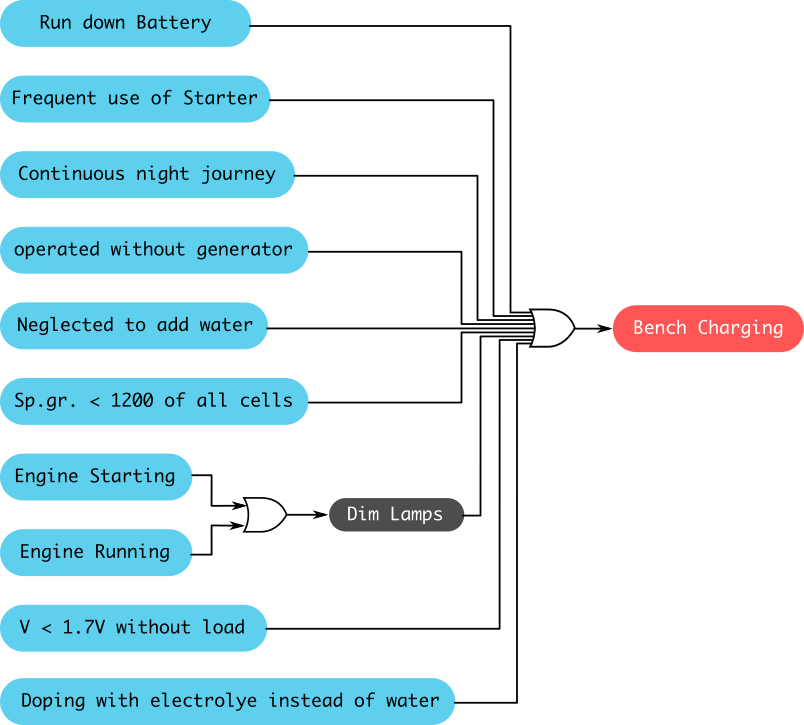
\includegraphics[width=0.7\linewidth]{./Resources/Images/conditions_benchcharge.png}
  \end{center}
\end{frame}

\begin{frame}     %----SLIDE
  \frametitle{How to Bench Charge ?}
  \fontsize{8pt}{10}\selectfont
  \begin{center}
    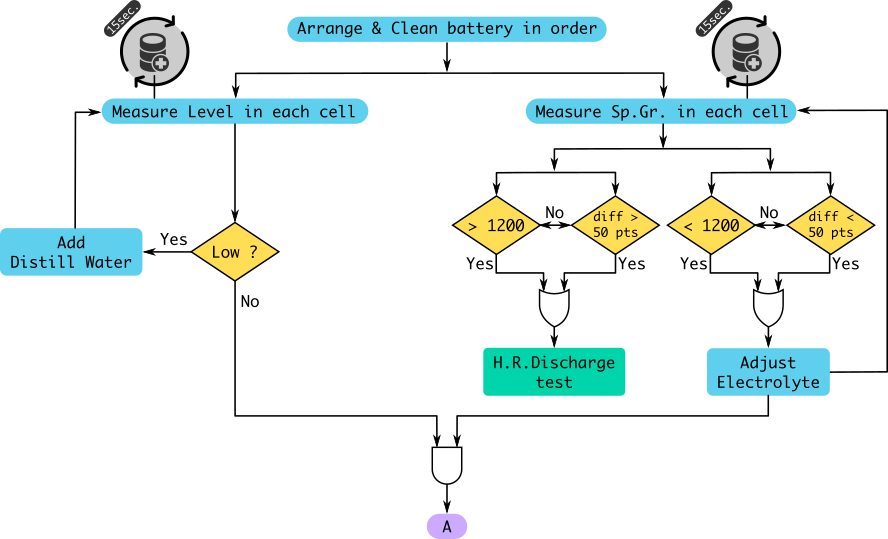
\includegraphics[width=\linewidth]{./Resources/Images/instructions_benchcharge_1.png}
  \end{center}
\end{frame}

\begin{frame}     %----SLIDE
  \frametitle{How to Bench Charge ? ...}
  \fontsize{8pt}{10}\selectfont
  \begin{center}
    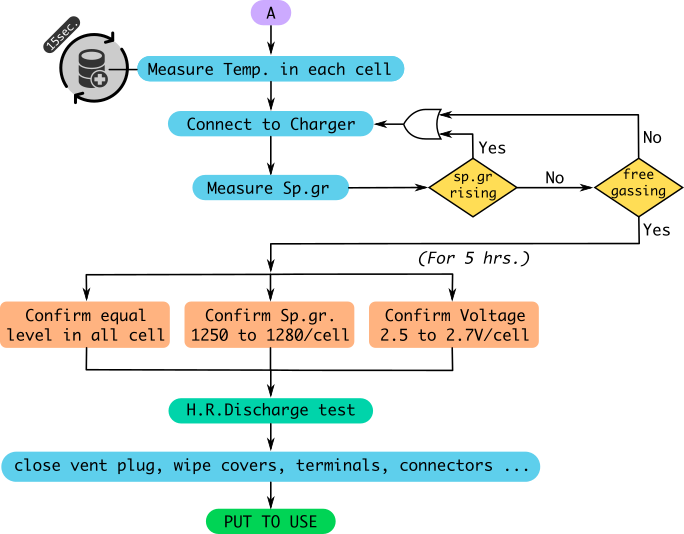
\includegraphics[width=0.85\linewidth]{./Resources/Images/instructions_benchcharge_2.png}
  \end{center}
\end{frame}

\begin{frame}     %----SLIDE
  \frametitle{Troubles while Bench Charging ...}
  \fontsize{8pt}{10}\selectfont
  \begin{itemize}
    \item Battery kept long time in discharging condition.
    \item Neglected to add water.
    \item Battery overheated by excessive charging rate.
    \item Shedded sediments causing short circuit of plates.
    \item Impurities attacking the plates and changes active materials to other substances.
    \item Separators may be clogged.
    \item Spongy lead may be bulged.
    \item Positive plates may be buckled.
    \item Sp.Gr. will not rise because of sediments - not enough to schort circuit.
    \item Sp.Gr. will not rise when impurities are added.
    \item Sp.Gr. will not rise when spilled electrolyte is replaced with water.
    \item Sp.Gr. will not rise when too much water is added.
    \item Battery will not hold charge due to impurities(ex: impure water).
    \item Battery will not hold charge due to shlow short circuit because of defective separators or excessive sediments.
  \end{itemize}
\end{frame}

\begin{frame}     %----SLIDE
  \frametitle{Probable Cause}
  \fontsize{7pt}{14}\selectfont
  \begin{itemize}
    \item \textbf{IF} : Sp.Gr. not raising to 1280  \\ \textbf{THEN} : make cadminum test; ascertain condition of plates 
    \item \textbf{IF} : one cell fails to charge \\ \textbf{CAUSE} : may be due to internal defect 
    \item \textbf{IF} : cells not take half a charge \\ \textbf{THEN} : battery is defective
    \item \textbf{IF} : Sp.Gr. is $>$ 1280 \\ \textbf{CAUSE} : doping of electrolyte  \\ \textbf{THEN} : refill with distilled water; charge for 10hrs twice; Fill back with 1250 Sp.Gr.
    \item \textbf{IF} : Hot on normal charging \\ \textbf{CAUSE} : badly sulfated; has partial short circuit 
    \item \textbf{IF} : electrolyte is milky white \\ \textbf{CAUSE} : presence of impurities 
  \end{itemize}
\end{frame}



\subsection{Testing}            %----SUBSECTION

{ % all template changes are local to this group.
    \setbeamertemplate{navigation symbols}{}
    \begin{frame}[plain]
        \begin{tikzpicture}[remember picture,overlay]
            \node[at=(current page.center)] {
                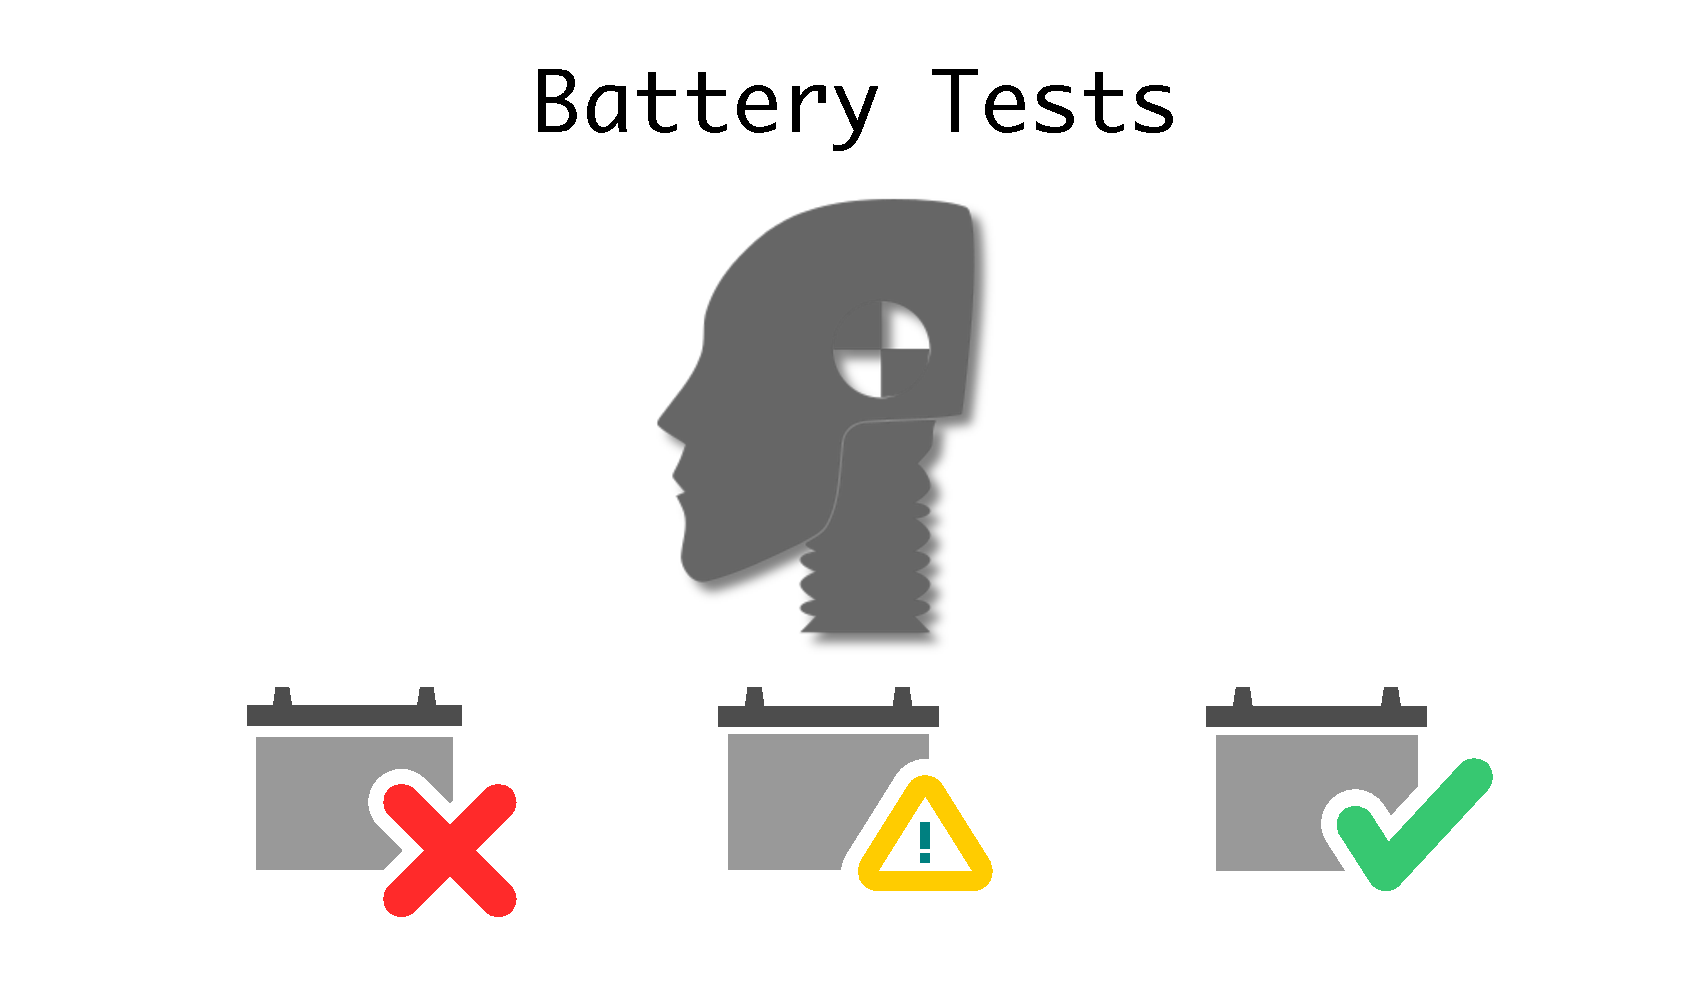
\includegraphics[width=\paperwidth]{./Resources/Images/Battery_Testing.pdf}
            };
        \end{tikzpicture}
     \end{frame}
}

\begin{frame}
  \frametitle{Tests conducted on Batteries}
  \fontsize{7pt}{10}\selectfont
  \textbf{\textit{Lighting ability Discharge test / CAPACITY TEST:}} Continuing for 5hrs. to a final voltage of 1.75V/cell, after charging for 24hrs. the battery discharges to 20\% of its 
  capacity - while readings are measured at 30min. interval.

  \bigskip
  \textbf{\textit{Starting ability Discharge test / HIGH RATE DISCHARGE TEST:}} After 24hrs. of fully charging in cold bath at -15\textcelsius, battery is discharged as per standard of 30sec. To 
  reach 9.1V and extends upto 6V of battery voltage at intervals of 5sec or 10sec. (@ 30sec. 9.1V is passed OK).
  
  \bigskip
  \textbf{\textit{Cycling Discharge test:}} New batteries are cyclically charged and discharged at the normal rates to come up the battery.
  
  \bigskip
  \textbf{\textit{Backup test:}} Conducted for invertor batteries after checking voltage, Sp.Gr. in each cell. Discharging at 200W or 400W as per standard of 13.2V for 100Ah or 150Ah for 
  2hrs.
  
  \bigskip
  \textbf{\textit{Life Cycle test:}} For all batteries (automotive/invertor) for 400 cycles 5hrs. charge at normal charging and 1hr discharge at 20A. For every 25 cycles batteries should
  be charged fully and capacity test to be conducted.
  
  \bigskip
  \textbf{\textit{Torque test:}} For automobile battery upto 400 cycles, 1.15hrs charge at 20A and 15min discharge at 80A. For every 50cycles battery fully charged and the capacity test 
  to be conducted.
\end{frame}

\begin{frame}
  \frametitle{General Tests}
  \fontsize{8pt}{12}\selectfont
  
  \textbf{General Inspection:} Helps in deciding what must be done.
  \begin{itemize}
    \item Is battery loose ?
    \item Are cables loose ?
    \item Is there corrosion at terminals ?
    \item Is top of battery wet ?
    \item Is top of case acid soaked ?
    \item Is lower part of case acid soaked ?
    \item Are ends of case bulged out ? - may be due to battery having been frozen.
  \end{itemize}
  
  \bigskip
  \textbf{Operation Tests:} Turn on the lights \& continue
  \begin{itemize}
    \item If its dim : then battery is run down or defective, may be put to bench charge.
    \item With lights burning and started switch to be closed, -- if the ight is very dim, the battery is run down or may be defective.
  \end{itemize}
\end{frame}

\begin{frame}
  \frametitle{General Tests ...}
  \fontsize{8pt}{12}\selectfont
  
  \textbf{Questioning the Driver/Battery man:}
  
  \bigskip
  \begin{itemize}
    \item Has water been added regularly ?
    \item Has impure water or river water ever been added to battery ?
    \item Has too much water been added ?
    \item Has electrolyte replaced by water ?
    \item Has battery been idle or stored without regular charging ?
    \item Is the vehicle operated at night than in day ?
    \item Is starter used frequently ?
    \item What is the average driving speed ?
    \item How long engine is usually cranked before starting ? (must not exceed 10 seconds).
  \end{itemize}
\end{frame}

\begin{frame}
  \frametitle{General Remedy}
  \fontsize{8pt}{10}\selectfont
  \renewcommand{\arraystretch}{1.5}
    \begin{tabularx}{\textwidth}{|X|X|X|}
    \hline
    \multicolumn{3}{|c|}{\textbf{ALL CELLS SHOW LOW GRAVITY OR LOW VOLTAGE}} \\
    \hline
    \textbf{\textit{Reason}} & \textbf{\textit{Problem}} & \textbf{\textit{Remedy}} \\
    \hline
    Loose/Dirty terminals & Reduced charging rate or open charging circuit & Tighten \& clean connections \\ \hline
    Corrosion on terminals & Reduced charging rate or open charging circuit & Clean corroded parts \& vaseline coated \\ \hline
    Broken terminals & Reduced charging rate or open charging circuit & Replace new terminals \\ \hline
    Generator not charging & -- & Replace the alternator \\ \hline
    Charging rate too low & -- & Replace the alternator \\ \hline
    Acid/moisture on top of battery & Causes corrosion and current leakage & Remove the things \\ \hline
    Short circuits in wiring & -- & Repair wiring \\ \hline
    \end{tabularx}
\end{frame}

\begin{frame}
  \frametitle{General Remedy ...}
  \fontsize{7.5pt}{10}\selectfont
  \renewcommand{\arraystretch}{1.3}
    \begin{tabularx}{\textwidth}{|X|X|X|}
    \hline
    \multicolumn{3}{|c|}{\textbf{GRAVITY READINGS UNEQUAL}} \\
    \hline
    \textbf{\textit{Reason}} & \textbf{\textit{Problem}} & \textbf{\textit{Remedy}} \\
    \hline
    Acid/moisture on top of battery & Causes current leakage & Remove cause \\ \hline
    Tools/wires on battery & Causing short circuits & Remove things  \\ \hline
    Electrolyte or acid added to cells & -- & --  \\ \hline
    Electrolyte spilled and replaced by water & -- &  \\ \hline
    Grooved side of separators placed against negatives & -- &  \\ \hline
    Cracked/leftout Separators & -- &  \\ \hline
    Old plates used in some cells and new in others & -- & --  \\ \hline
    Impurities in cells & Low Gravity & --  \\ \hline
    Shorted Cell & -- & -- \\ \hline
    Cracked Jar & -- & -- \\ \hline
    \end{tabularx}
\end{frame}

\begin{frame}
  \frametitle{Care to be taken by Electrician}
  \fontsize{8pt}{10}\selectfont
  \begin{itemize}
    \item Alternator must be checked frequently for output. Worn out bearings, carbon brushes must be replaced.
    \item Fan belt checkup and to be replaced on scheduled manner.
    \item Fan belt tension must be checked in frequent intervals.
    \item After fan belt replacement or end routes breakdown or alternator breakdown - a bench charge is advisable.
    \item If fault is ascertained with starter - would run down the battery - replace immediately.
    \item Damaged braided copper strip may be replaced.
    \item It is advisable that whenever FC or half FC all connections should be checked and replaced when required.
    \item Whenever starter or alternator received for reconditioning, essentials like bearings, carbon brushes must be replaced without fail.
    \item A perfect record of topup, bench charging and replacement of alternator or starter should be maintained for each vehicle.
    \item Whenever the vehicle is kept idle for more than 2 days, the battery may be charged in bench.
    \item It is best practice to make bench charging every 6 months.
  \end{itemize}
\end{frame}



%--------------------------------------------------
% Credits :)
%--------------------------------------------------

\section{credits}

\begin{frame}
\frametitle{Credits}
\fontsize{7.5pt}{12}\selectfont
\centering
This Document Contains lot of icons, taken from collaborative internet web sites \\ 
which offer the content under CC license. \\
\bigskip

Since every icons in each block diagram cannot be attributed seperately\\
So i am providing the link where it can be from. \\

\begin{figure}[h]
\centering
      \href{https://thenounproject.com/}{
\includegraphics[width=0.2\linewidth]{./Resources/Images/urllink.png}}
\end{figure}
\end{frame}

\begin{frame}
  \fontsize{50pt}{12}\selectfont
  \begin{center}
    Thank you !
  \end{center}
\end{frame}

\end{document} 
 
